% !TEX root = ../zavrsni_rad.tex

\chapter{Rezultati i evaluacija}
\label{pog:rezultati}

U ovom poglavlju prikazano je kako se sustav ponaša u praksi. Za svaki od sedam testnih scenarija prikazane su trajektorija robota, upravljački signali i greška praćenja, te su izmjereni pokazatelji kvalitete. Nakon toga analizirano je kako promjena dva ključna parametra sustava --- predikcijskog horizonta $N$ i težina troška --- utječe na preciznost i brzinu izvođenja. Poglavlje završava tablicom usporedbe svih scenarija.

\FloatBarrier
% ─────────────────────────────────────────────────────────────────────────────
\section{Eksperimentalni postav}
\label{sec:r_postav}

Sva ispitivanja provedena su u simulacijskom okruženju implementiranom u Pythonu, korištenjem acados solvera za rješavanje OCP-a. Simulacijsko okruženje modelira ravnu površinu dimenzija $10\ \text{m} \times 10\ \text{m}$. Simulacija se odvija u zatvorenoj petlji s korakom uzorkovanja $\Delta t = 0{,}1$ s i završava kada robot dođe unutar $d_{tol} = 0{,}3$ m od cilja ili po isteku $k_{max} = 1000$ koraka. Metrike evaluacije definirane su u poglavlju~\ref{pog:implementacija}, a pregled testnih scenarija u tablici~\ref{tab:scenariji}.

Sva mjerenja izvršena su na prijenosnom računalu s procesorom Intel Core 7 150U i 32 GB RAM-a, pod operacijskim sustavom Fedora 42 (Linux kernel 6.19.14). Korišteni softver: Python 3.13.13, acados 0.5.1, CasADi 3.7.2, SciPy 1.17.1; solver je kompajliran kompajlerom GCC 15.2.1. CPU vrijeme jednog koraka mjereno je funkcijom \texttt{time.perf\_counter()} neposredno oko poziva \texttt{solver.solve()} (prikazano u listingu u poglavlju~\ref{pog:implementacija}).

Tablica~\ref{tab:params} prikazuje sve ključne parametre korištene u eksperimentima.

\begin{table}[H]
\centering
\caption{Parametri simulacijskog okruženja}
\label{tab:params}
\begin{tabular}{llll}
\toprule
Skupina & Parametar & Oznaka & Vrijednost \\
\midrule
\textbf{Robot} & Polumjer & $r_{rob}$ & $0{,}2$ m \\
 & Maksimalna brzina & $v_{max}$ & $1{,}0$ m/s \\
 & Minimalna brzina & $v_{min}$ & $0{,}05$ m/s \\
 & Maksimalna kutna brzina & $\omega_{max}$ & $1{,}5$ rad/s \\
 & Maks.\ translacijsko ubrzanje & $a_{v,max}$ & $0{,}5$ m/s\textsuperscript{2} \\
 & Maks.\ kutno ubrzanje & $\alpha_{max}$ & $1{,}0$ rad/s\textsuperscript{2} \\
\midrule
\textbf{NMPC} & Predikcijski horizont & $N$ & 20 koraka \\
 & Korak uzorkovanja & $\Delta t$ & $0{,}1$ s \\
 & Težine pozicije & $Q_x, Q_y$ & $10{,}0$ \\
 & Težina orijentacije & $Q_\theta$ & $1{,}0$ \\
 & Terminalna težinska matrica & $W_e$ & $Q$ \\
 & Težine upravljanja & $R_{a_v}, R_{\alpha}$ & $0{,}1$ \\
 & Vrsta ograničenja prepreka & — & meka (soft) \\
 & Vrsta solvera & — & SQP\_RTI \\
\midrule
\textbf{A*} & Rezolucija mreže & $d_{grid}$ & $0{,}2$ m \\
 & Ukupna inflacija prepreka & $d_{inf}$ & $0{,}4$ m ($0{,}2$ sigurnost $+$ $0{,}2$ polumjer) \\
\midrule
\textbf{Simulacija} & Tolerancija cilja & $d_{tol}$ & $0{,}3$ m \\
 & Integrator & — & RK4 \\
 & Maks.\ broj koraka & $k_{max}$ & $1000$ \\
\bottomrule
\end{tabular}
\end{table}

Konfiguracija je pohranjena u datoteci \texttt{config/params.yaml}:

\begin{listing}[H]
\begin{minted}{yaml}
robot:
  radius: 0.2
  v_max: 1.0
  v_min: 0.05
  omega_max: 1.5
  dv_max: 0.5
  domega_max: 1.0
mpc:
  N: 20
  dt: 0.1
  Q: [10.0, 10.0, 1.0]
  R: [0.1, 0.1]
  solver_type: SQP_RTI
  constraints: soft
simulation:
  goal_tolerance: 0.3
  max_steps: 1000
\end{minted}
\caption{Ključni parametri u \texttt{config/params.yaml}}
\end{listing}

\FloatBarrier
% ─────────────────────────────────────────────────────────────────────────────
\section{Osnovna putanja}
\label{sec:r_baseline}

Scenarij osnovne putanje definira kretanje od $(0{,}5;\; 0{,}5)$ s orijentacijom $\theta_0 = 0$ do cilja $(9{,}5;\; 9{,}5)$, bez prepreka. Svrha je provjera ispravnosti sustava u idealnim uvjetima i uspostava referentnih vrijednosti za usporedbu s kompleksnijim scenarijima. A* planira dijagonalnu putanju koju algoritam glađenja pretvara u glatku krivulju duljine oko 12,7 m.

\begin{figure}[htbp]
  \centering
  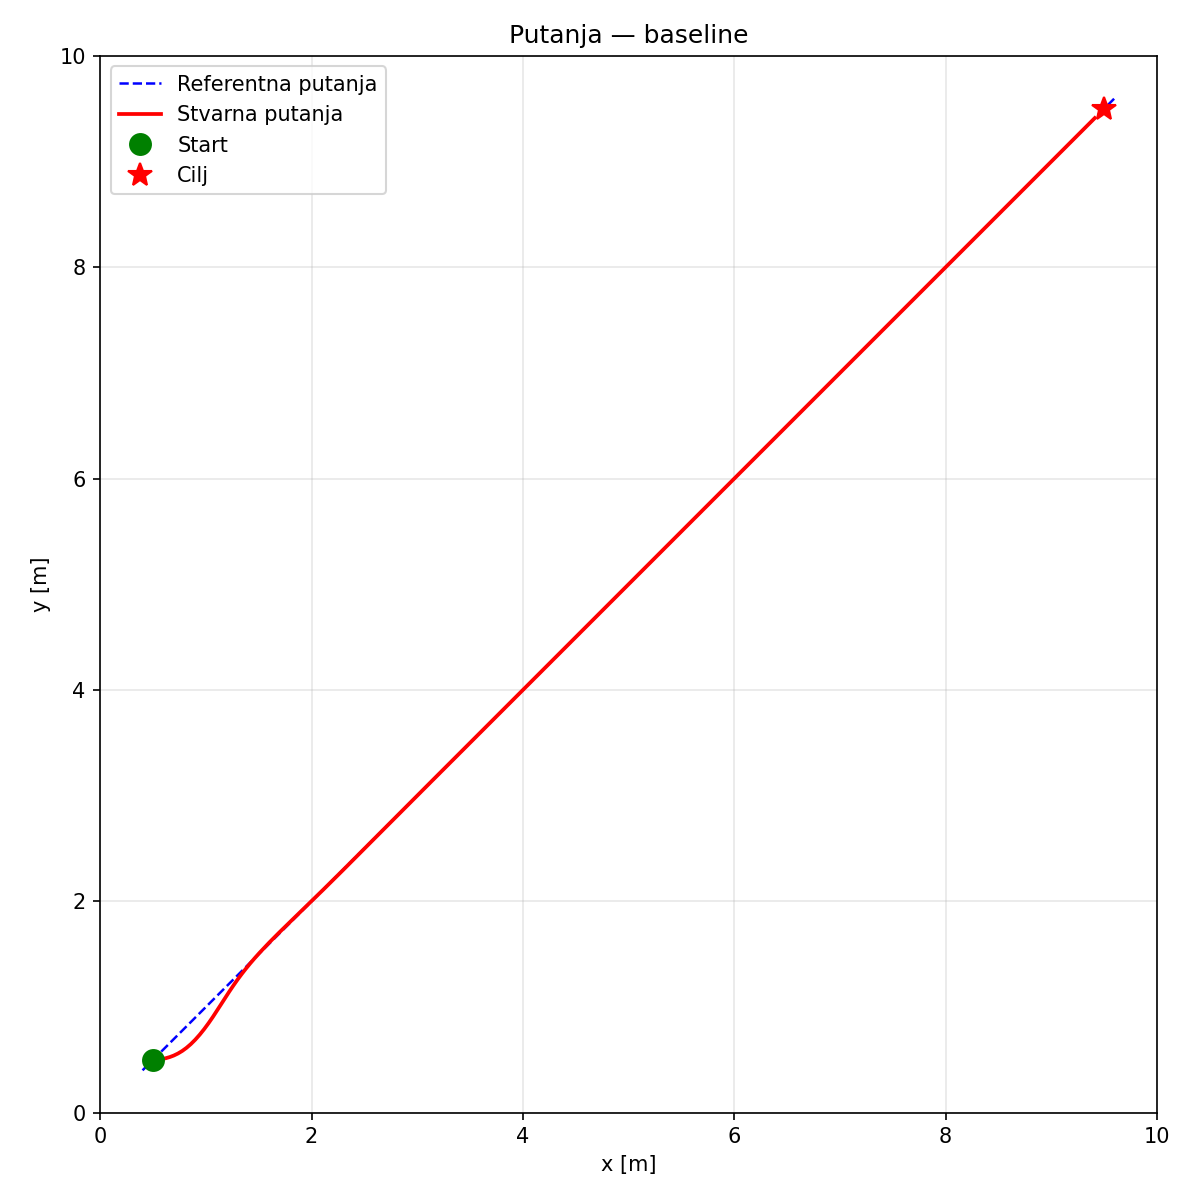
\includegraphics[width=0.82\linewidth]{figures/baseline_traj.png}
  \caption{Referentna i stvarna putanja robota u scenariju bez prepreka.}
  \label{slk:baseline_traj}
\end{figure}

Slika~\ref{slk:baseline_traj} pokazuje da stvarna putanja prati referentnu s RMSE od $34{,}4$ mm. Jedino vidljivo odstupanje pojavljuje se na početku kretanja gdje robot s $\theta_0 = 0$ mora korigirati smjer prema dijagonalnom referentnom pravcu (kut $\approx 45°$). NMPC regulator ispravno prepoznaje taj zahtjev i robota glatko preusmjerava bez oscilacija.

\begin{figure}[htbp]
  \centering
  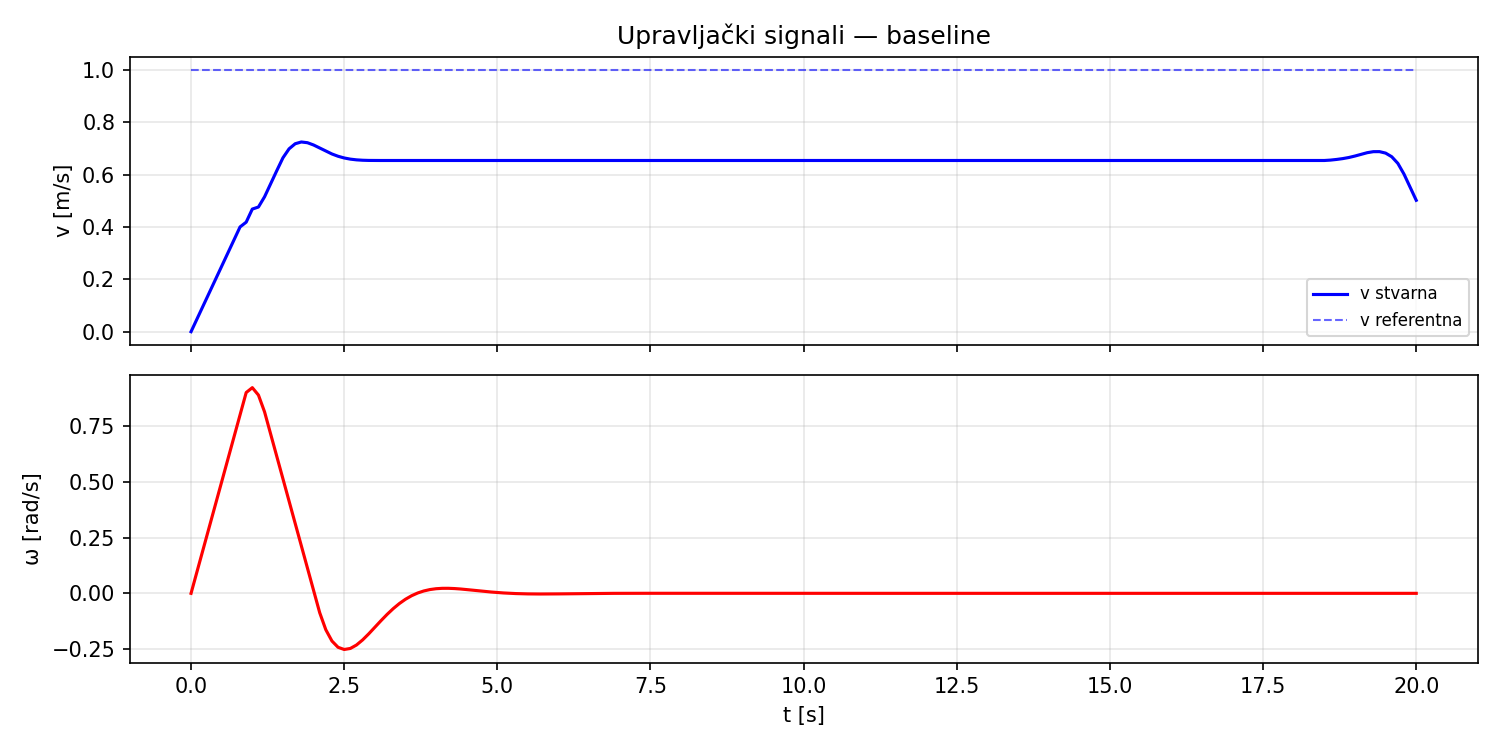
\includegraphics[width=0.82\linewidth]{figures/baseline_controls.png}
  \caption{Brzina $v(t)$ i kutna brzina $\omega(t)$ u scenariju bez prepreka.}
  \label{slk:baseline_controls}
\end{figure}

Graf upravljačkih signala (slika~\ref{slk:baseline_controls}) potvrđuje ispravno ponašanje: brzina $v$ raste do $v_{max} = 1{,}0$ m/s i ostaje na toj razini do blizine cilja, dok kutna brzina $\omega$ pokazuje vrh od $\approx 0{,}87$ rad/s u prvoj sekundi (inicijalna korekcija smjera), a potom se stabilizira blizu nule.

\begin{figure}[htbp]
  \centering
  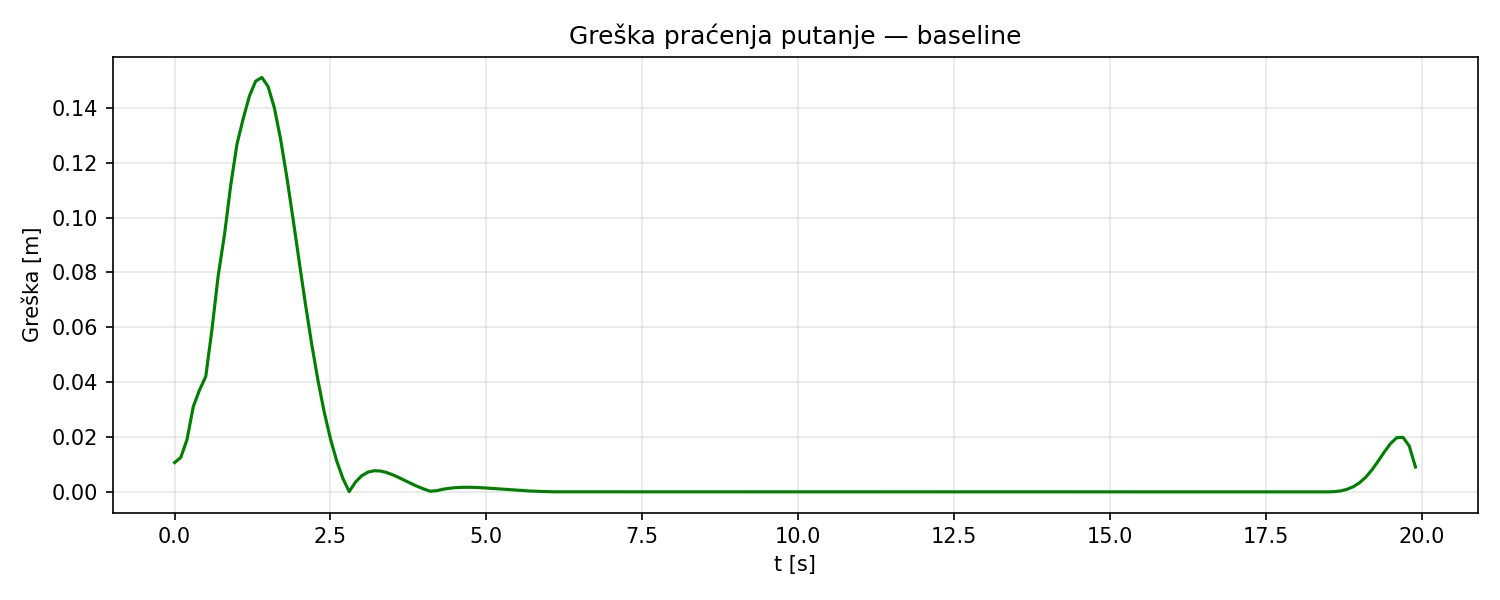
\includegraphics[width=0.82\linewidth]{figures/baseline_error.png}
  \caption{Greška praćenja u funkciji vremena za scenarij bez prepreka.}
  \label{slk:baseline_error}
\end{figure}

Graf greške (slika~\ref{slk:baseline_error}) prikazuje maksimum od $\approx 0{,}15$ m oko $t \approx 1{,}5$ s, što odgovara inicijalnoj korekciji smjera, a potom brzo opada ispod $0{,}03$ m.

\begin{table}[H]
\centering
\caption{Metrike --- osnovna putanja}
\label{tab:baseline}
\begin{tabular}{ll}
\toprule
Metrika & Vrijednost \\
\midrule
RMSE & $0{,}0344$ m \\
CTE srednji & $0{,}0107$ m \\
CTE max & $0{,}1478$ m \\
Greška smjera (srednja) & $2{,}73°$ \\
Vrijeme do cilja & $20{,}00$ s \\
CPU (prosjek / max) & $0{,}091$ ms / $0{,}319$ ms \\
Dostigao cilj & Da \\
\bottomrule
\end{tabular}
\end{table}

RMSE od $34{,}4$ mm i srednja bočna greška od $10{,}7$ mm potvrđuju visoku kvalitetu praćenja. Prosječno CPU vrijeme od $0{,}091$ ms po koraku iznosi manje od $0{,}1$\% trajanja uzornog intervala od $100$ ms, što pokazuje da je sustav primjenjiv u stvarnim uvjetima gdje je vrijeme odziva ključno.

\FloatBarrier
% ─────────────────────────────────────────────────────────────────────────────
\section{Jedna prepreka}
\label{sec:r_one_obstacle}

Scenarij uvodi kružnu prepreku polumjera $r = 1{,}0$ m u središte prostora u točki $(5{,}0;\; 5{,}0)$. Robot kreće iz $(0{,}5;\; 0{,}5)$ prema cilju $(9{,}5;\; 9{,}5)$, pa prepreka direktno blokira najkraću dijagonalnu putanju. A* pronalazi put koji zaobilazi prepreku s gornje lijeve strane.

\begin{figure}[htbp]
  \centering
  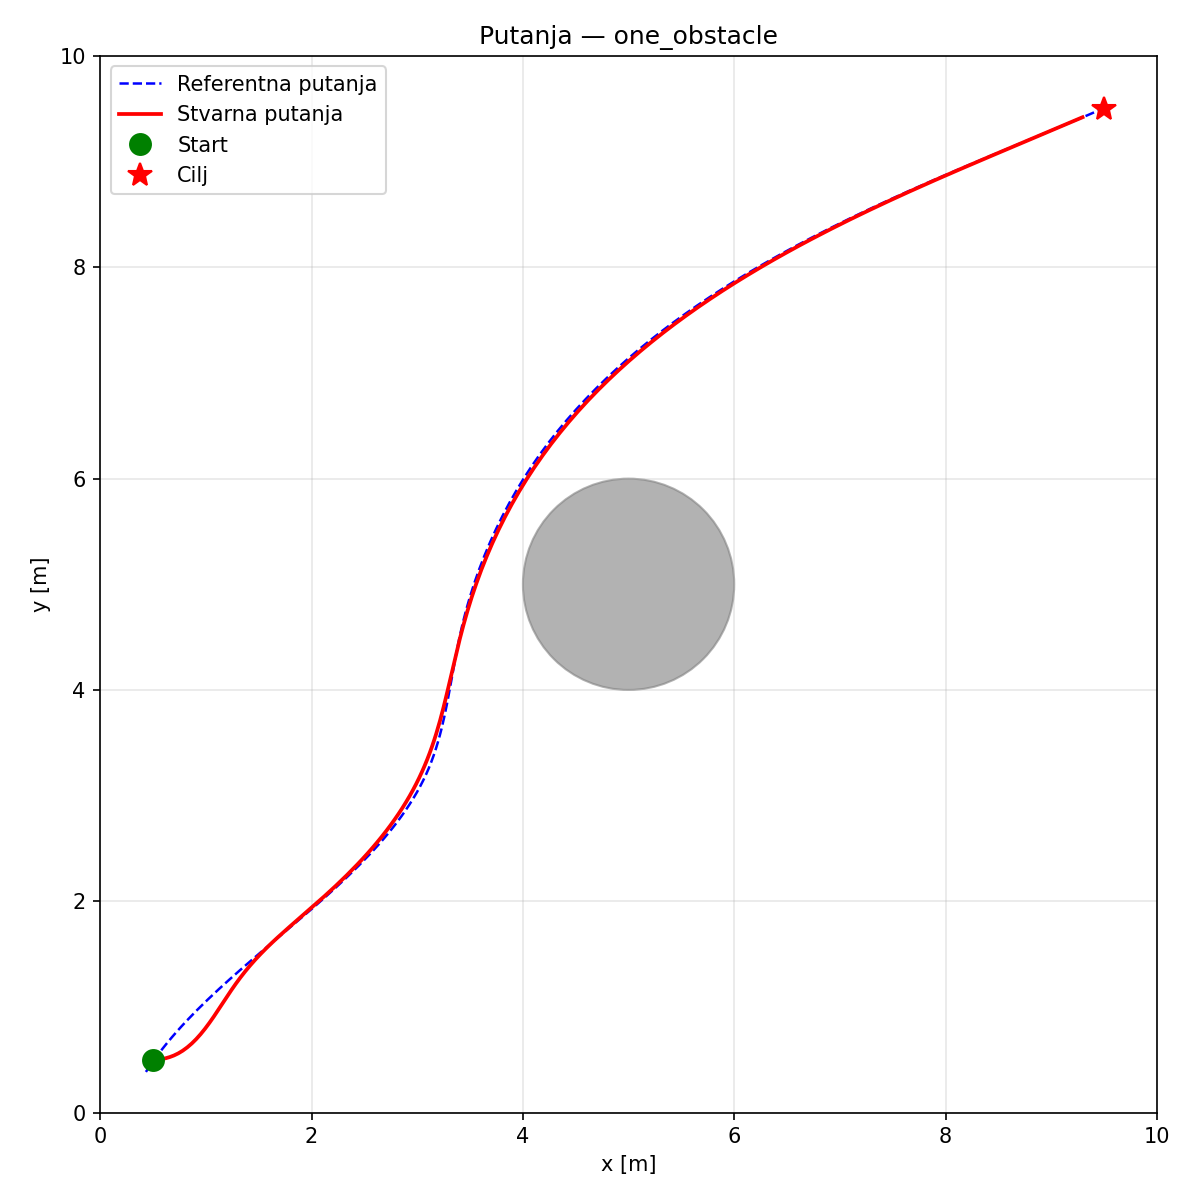
\includegraphics[width=0.82\linewidth]{figures/one_obstacle_traj.png}
  \caption{Referentna i stvarna putanja u scenariju s jednom kružnom preprekom. Robot zaobilazi prepreku s gornje lijeve strane.}
  \label{slk:one_obstacle_traj}
\end{figure}

Slika~\ref{slk:one_obstacle_traj} pokazuje da robot prati referentnu putanju s visokom točnošću, uključujući zavoj oko prepreke. Minimalna udaljenost od ruba prepreke iznosi više od $0{,}4$ m, što je iznad zbroja polumjera robota i sigurnosne margine, pa meka ograničenja prepreka u NMPC-u nisu bila aktivna.

\begin{figure}[htbp]
  \centering
  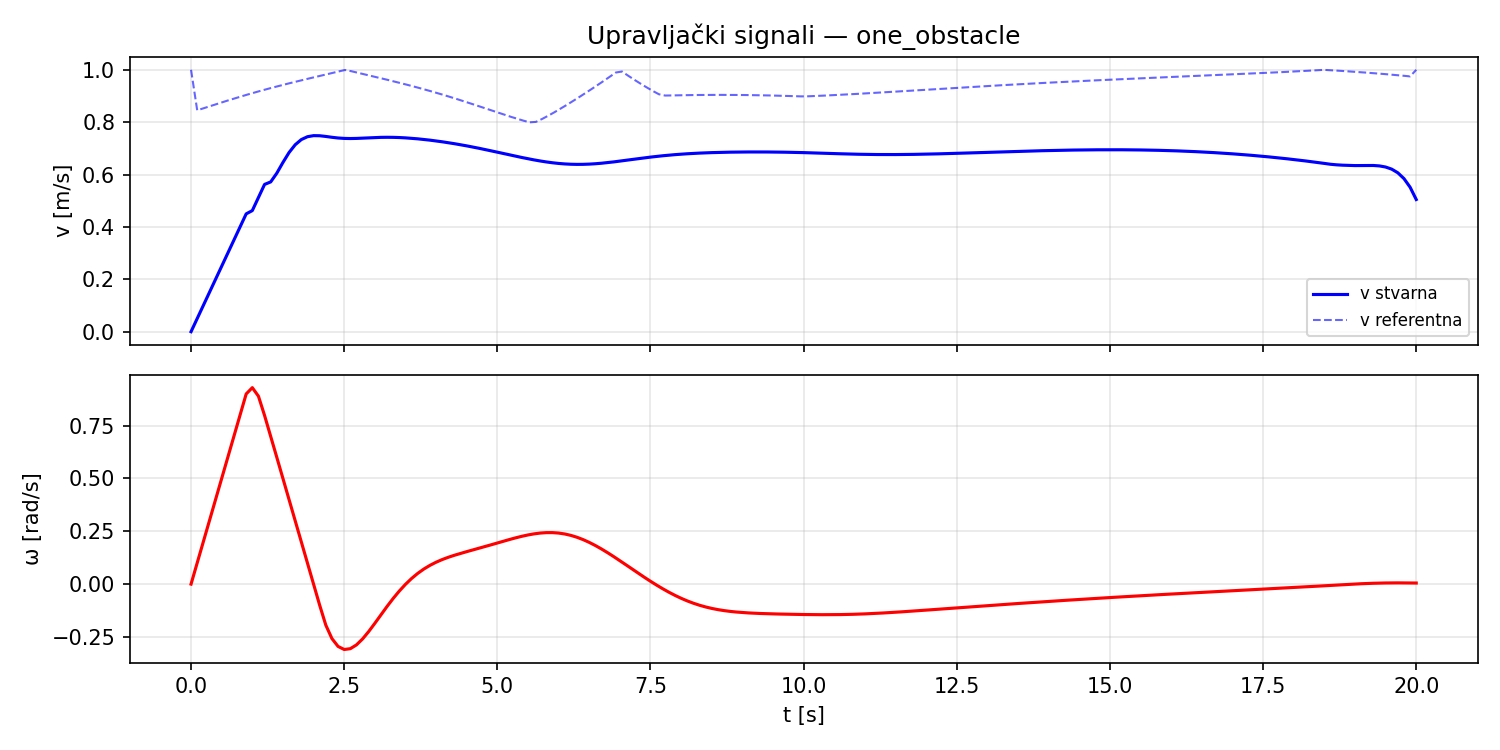
\includegraphics[width=0.82\linewidth]{figures/one_obstacle_controls.png}
  \caption{Brzina $v(t)$ i kutna brzina $\omega(t)$ u scenariju s jednom preprekom. Dva karakteristična vrha $\omega$ odgovaraju inicijalnoj korekciji smjera i zavoju oko prepreke.}
  \label{slk:one_obstacle_controls}
\end{figure}

\begin{figure}[htbp]
  \centering
  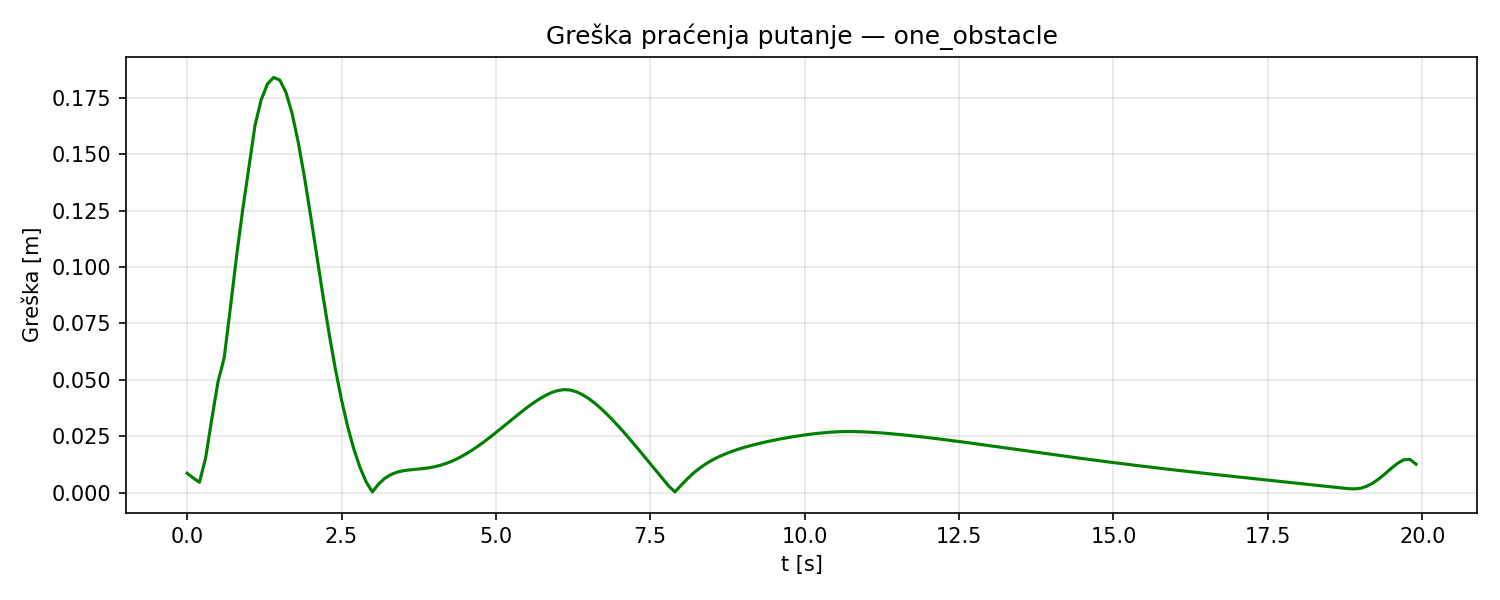
\includegraphics[width=0.82\linewidth]{figures/one_obstacle_error.png}
  \caption{Greška praćenja u scenariju s jednom preprekom.}
  \label{slk:one_obstacle_error}
\end{figure}

\begin{table}[H]
\centering
\caption{Metrike --- jedna prepreka}
\label{tab:one_obstacle}
\begin{tabular}{lll}
\toprule
Metrika & Vrijednost & Usporedba s osnovnim \\
\midrule
RMSE & $0{,}0469$ m & $+36{,}1$\% \\
CTE srednji & $0{,}0278$ m & $+160{,}7$\% \\
CTE max & $0{,}1839$ m & $+24{,}4$\% \\
Greška smjera (srednja) & $3{,}87°$ & $+42{,}0$\% \\
Vrijeme do cilja & $20{,}00$ s & $0$\% \\
CPU (prosjek / max) & $0{,}099$ ms / $0{,}359$ ms & $+8{,}8$\% \\
Dostigao cilj & Da & --- \\
\bottomrule
\end{tabular}
\end{table}

RMSE i CTE su veći nego u osnovnom scenariju jer putanja sada ima zavoj oko prepreke --- robot ne može trenutačno promijeniti smjer pa u krivini blago zaostaje za referencom. Unatoč tome, RMSE ostaje ispod $50$ mm, a dodatno CPU opterećenje ($+8{,}8$\%) je zanemarivo.

\FloatBarrier
% ─────────────────────────────────────────────────────────────────────────────
\section{Uski prolaz}
\label{sec:r_narrow}

Scenarij postavlja dvije kružne prepreke polumjera $r = 1{,}2$ m u točkama $(5{,}0;\; 3{,}5)$ i $(5{,}0;\; 6{,}5)$. Robot kreće iz $(0{,}5;\; 5{,}0)$ prema $(9{,}5;\; 5{,}0)$, pa referentna putanja prolazi upravo između tih prepreka.

Geometrijska analiza otkriva ključnu karakteristiku scenarija: uzimajući u obzir ukupnu inflaciju od $d_{inf} = 0{,}4$ m (sigurnosna margina $0{,}2$ m $+$ polumjer robota $0{,}2$ m), efektivna širina prolaza između infliranih prepreka iznosi:
\begin{equation}
  d_{prolaz} = (6{,}5 - 1{,}2 - 0{,}4) - (3{,}5 + 1{,}2 + 0{,}4) = 4{,}9 - 5{,}1 = -0{,}2 \text{ m}
\end{equation}

Negativna vrijednost znači da prolaz između prepreka nije prohodan za robota. A* zato planira put koji zaobilazi donju prepreku ispod nje, spuštajući putanju do $y \approx 2{,}2$ m.

\begin{figure}[htbp]
  \centering
  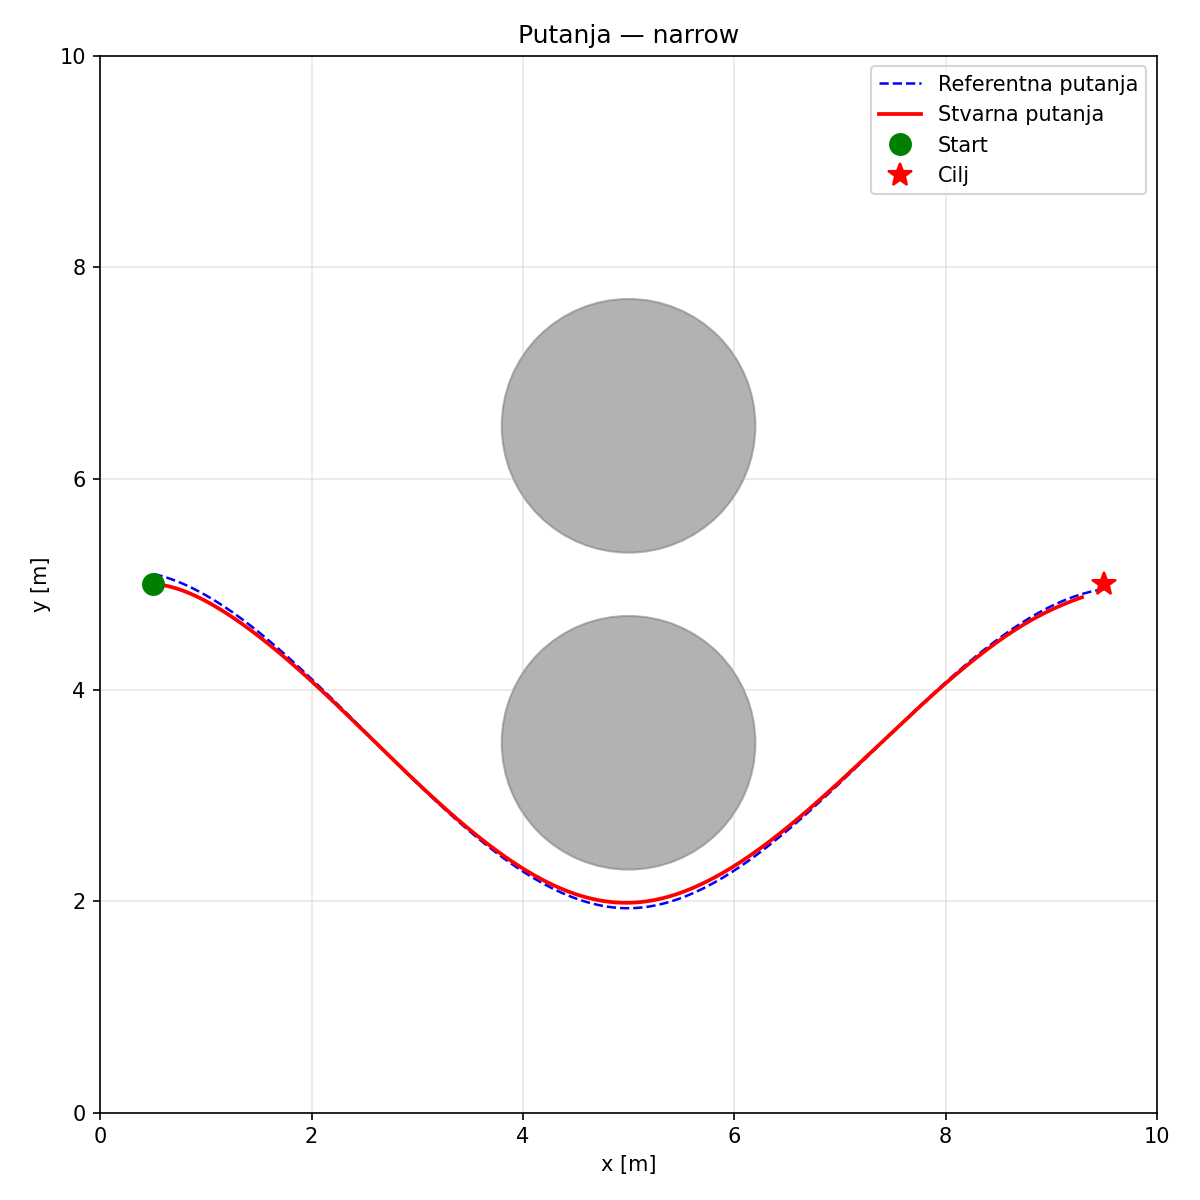
\includegraphics[width=0.82\linewidth]{figures/narrow_traj.png}
  \caption{Referentna i stvarna putanja u scenariju uskog prolaza. A* planira put ispod donje prepreke jer je prolaz između njih blokiran proširenim područjem prepreka.}
  \label{slk:narrow_traj}
\end{figure}

Slika~\ref{slk:narrow_traj} prikazuje karakteristični luk: robot se spušta prema jugu, prolazi ispod donje prepreke pri $y \approx 2{,}2$ m, a zatim se vraća prema ciljnoj koordinati $y = 5{,}0$ m. Robot prati zadanu putanju s visokom točnošću, a minimalna udaljenost od ruba donje prepreke iznosi oko $0{,}5$ m.

\begin{figure}[htbp]
  \centering
  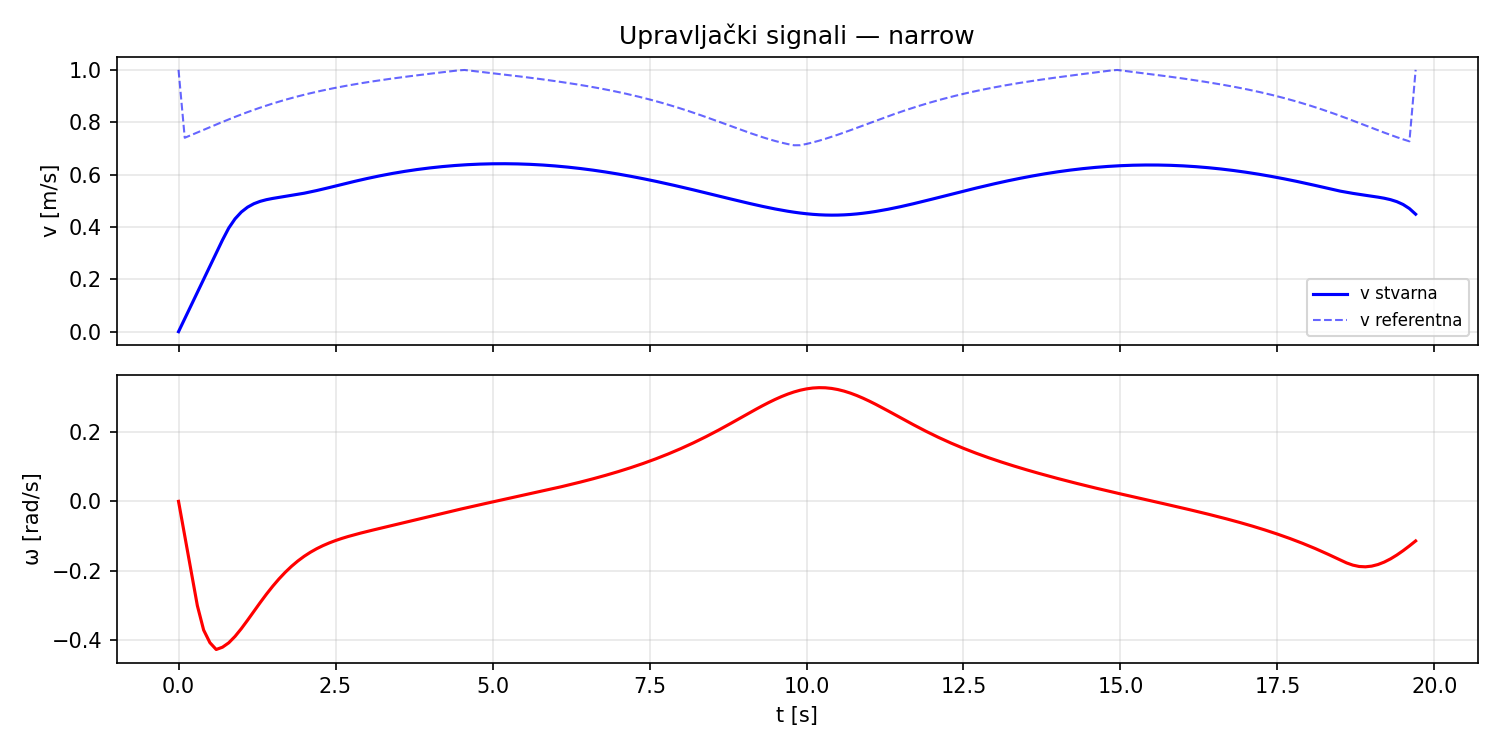
\includegraphics[width=0.82\linewidth]{figures/narrow_controls.png}
  \caption{Brzina $v(t)$ i kutna brzina $\omega(t)$ u scenariju uskog prolaza. Kontinuirani sinusoidalni profil $\omega$ odgovara zaobilaženju prepreke.}
  \label{slk:narrow_controls}
\end{figure}

\begin{figure}[htbp]
  \centering
  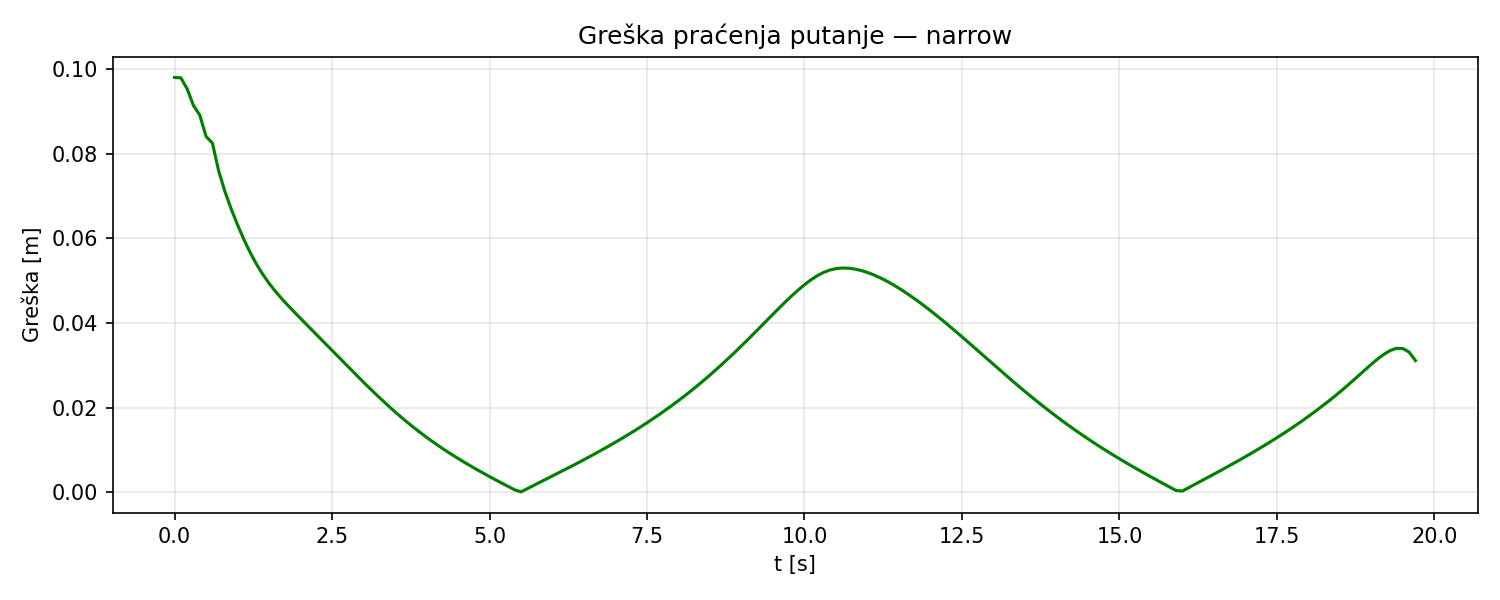
\includegraphics[width=0.82\linewidth]{figures/narrow_error.png}
  \caption{Greška praćenja u scenariju uskog prolaza. Dva područja povišene greške odgovaraju dvjema najizraženijim krivinama putanje.}
  \label{slk:narrow_error}
\end{figure}

\begin{table}[H]
\centering
\caption{Metrike --- uski prolaz}
\label{tab:narrow}
\begin{tabular}{lll}
\toprule
Metrika & Vrijednost & Usporedba s osnovnim \\
\midrule
RMSE & $0{,}0344$ m & $\approx 0$\% \\
CTE srednji & $0{,}0270$ m & $+152{,}7$\% \\
CTE max & $0{,}0962$ m & $-34{,}9$\% \\
Greška smjera (srednja) & $1{,}59°$ & $-41{,}5$\% \\
Vrijeme do cilja & $19{,}70$ s & $-1{,}5$\% \\
CPU (prosjek / max) & $0{,}089$ ms / $0{,}263$ ms & $-2{,}2$\% \\
Dostigao cilj & Da & --- \\
\bottomrule
\end{tabular}
\end{table}

Ostvareni RMSE ($34{,}4$ mm) jednak je onom iz osnovnog scenarija, a greška smjera ($1{,}59°$) je najmanji od svih scenarija. Razlog je jednostavan: robot kreće s početnom orijentacijom $\theta_0 = 0$ (prema desno) i cilj se nalazi upravo u tom smjeru, pa ne treba inicijalna korekcija kuta --- za razliku od osnovnog scenarija gdje je robot morao odmah skrenuti za $\approx 45°$.

\FloatBarrier
% ─────────────────────────────────────────────────────────────────────────────
\section{L-hodnik}
\label{sec:r_lcorridor}

U ovom scenariju velik pravokutni zid dimenzija $7{,}5\ \text{m} \times 6{,}5\ \text{m}$ blokira gornji lijevi dio prostora. Robot mora prijeći karakteristični L-oblik putanje: horizontalni prolaz duž donjeg ruba prepreke, a potom okret za $90°$ i vertikalni uspon uz njezin desni rub.

\begin{figure}[htbp]
  \centering
  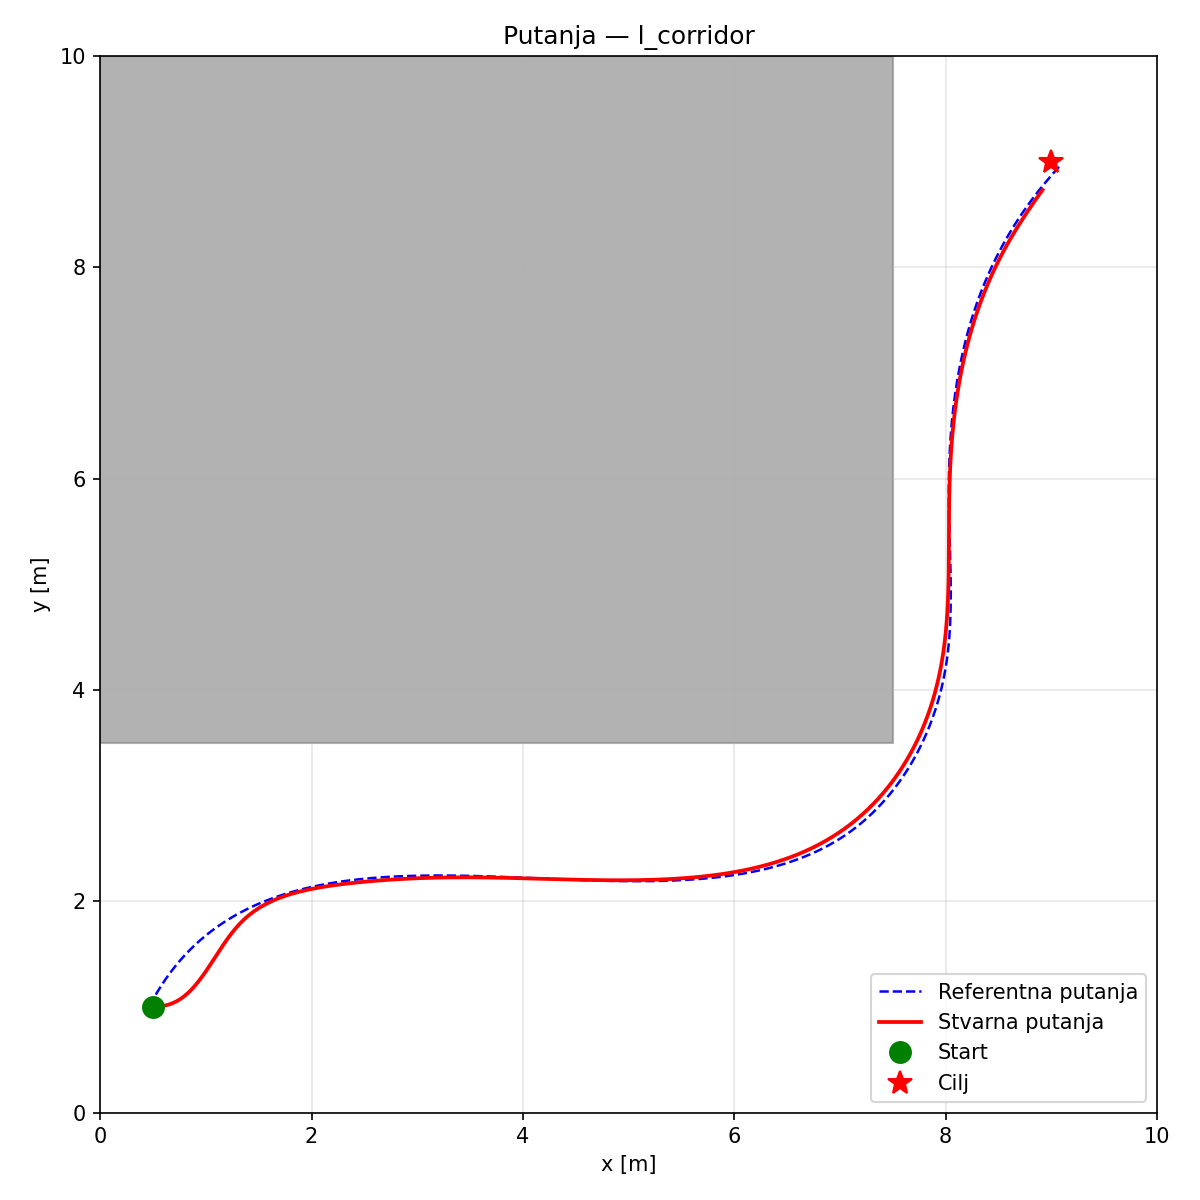
\includegraphics[width=0.82\linewidth]{figures/l_corridor_traj.png}
  \caption{Referentna i stvarna putanja u scenariju L-hodnika. Pravokutna prepreka (siva površina) prisiljava robota na L-oblik putanje.}
  \label{slk:lcorridor_traj}
\end{figure}

\begin{figure}[htbp]
  \centering
  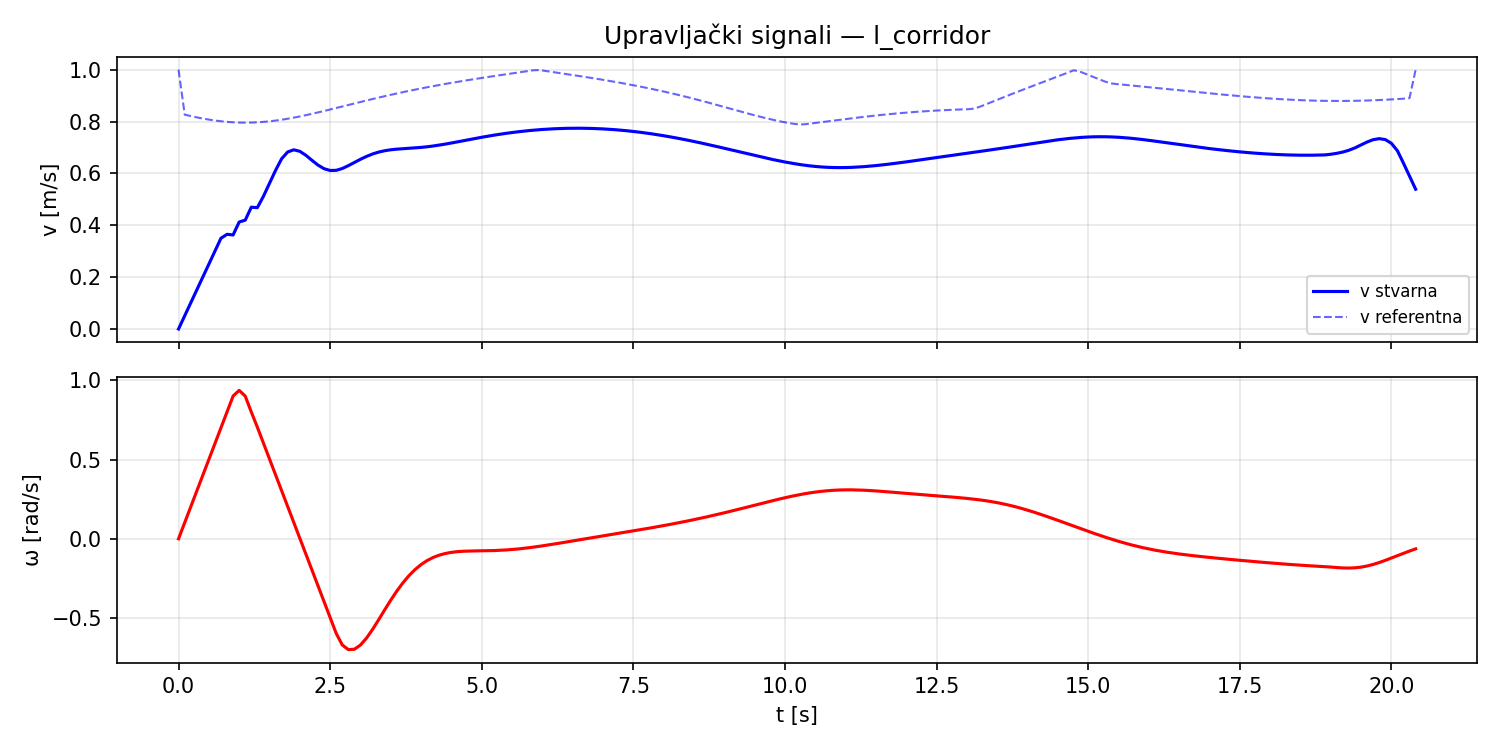
\includegraphics[width=0.82\linewidth]{figures/l_corridor_controls.png}
  \caption{Brzina $v(t)$ i kutna brzina $\omega(t)$ u scenariju L-hodnika. Negativni vrh $\omega \approx -1{,}0$ rad/s oko $t \approx 2{,}8$ s odgovara oštrom zaokretu na kraju horizontalnog dijela.}
  \label{slk:lcorridor_controls}
\end{figure}

Kutna brzina dostiže $\omega_{min} \approx -1{,}0$ rad/s, što je blizu ograničenja $\omega_{max} = 1{,}5$ rad/s i pokazuje da robot mora skrenuti gotovo maksimalnom kutnom brzinom kako bi prošao oštar ugao hodnika.

\begin{figure}[htbp]
  \centering
  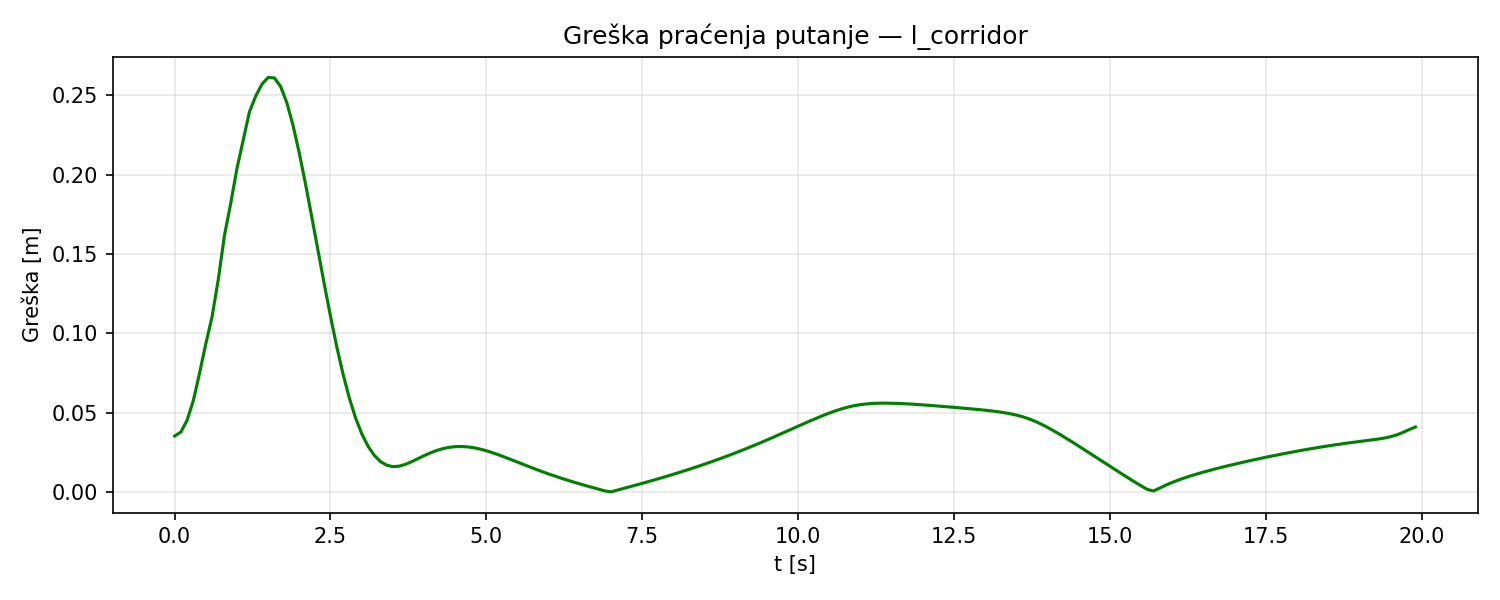
\includegraphics[width=0.82\linewidth]{figures/l_corridor_error.png}
  \caption{Greška praćenja u scenariju L-hodnika. Inicijalni vrh od $0{,}285$ m najveći je u svim pravilnim scenarijima.}
  \label{slk:lcorridor_error}
\end{figure}

\begin{table}[H]
\centering
\caption{Metrike --- L-hodnik}
\label{tab:lcorridor}
\begin{tabular}{lll}
\toprule
Metrika & Vrijednost & Usporedba s osnovnim \\
\midrule
RMSE & $0{,}0724$ m & $+110{,}2$\% \\
CTE srednji & $0{,}0457$ m & $+328{,}3$\% \\
CTE max & $0{,}2610$ m & $+76{,}6$\% \\
Greška smjera (srednja) & $4{,}90°$ & $+79{,}7$\% \\
Vrijeme do cilja & $20{,}40$ s & $+2{,}0$\% \\
CPU (prosjek / max) & $0{,}103$ ms / $0{,}251$ ms & $+13{,}2$\% \\
Dostigao cilj & Da & --- \\
\bottomrule
\end{tabular}
\end{table}

Najveći inicijalni vrh greške ($0{,}285$ m) nastaje kombinacijom greške pozicije i greške smjera na startu --- robot stoji na $y = 1{,}0$ m s $\theta_0 = 0$, dok referentna putanja odmah skreće prema $y \approx 2{,}2$ m. Bez tog prijelaznog odziva prosječna greška u oba segmenta hodnika bila bi usporediva s jednostavnijim scenarijima.

\FloatBarrier
% ─────────────────────────────────────────────────────────────────────────────
\section{U-oblik}
\label{sec:r_ushape}

Tri pravokutne prepreke formiraju slijepu ulicu otvorenu prema jugu: lijeva stranica, desna stranica i gornja stranica U-oblika. Robot polazi iz $(5{,}0;\; 0{,}5)$ s $\theta_0 = \pi/2$ i mora doseći cilj $(5{,}0;\; 9{,}5)$, koji se nalazi izravno iza gornje stranice U. Naivni pristup prema cilju odveo bi robota ravno u zamku.

Scenarij demonstrira neophodnost dvoslojne arhitekture: A* koji vidi cijeli prostor odjednom pronalazi jedini prohodani put --- zaobilazeći U-oblik izvana s desne strane. NMPC s horizontom $N = 20$ (predikcija $= 2$ s) pak ne može sam zaključiti o topologiji zamke, pa bi bez globalne reference mogao zaglaviti unutar U-oblika.

\begin{figure}[htbp]
  \centering
  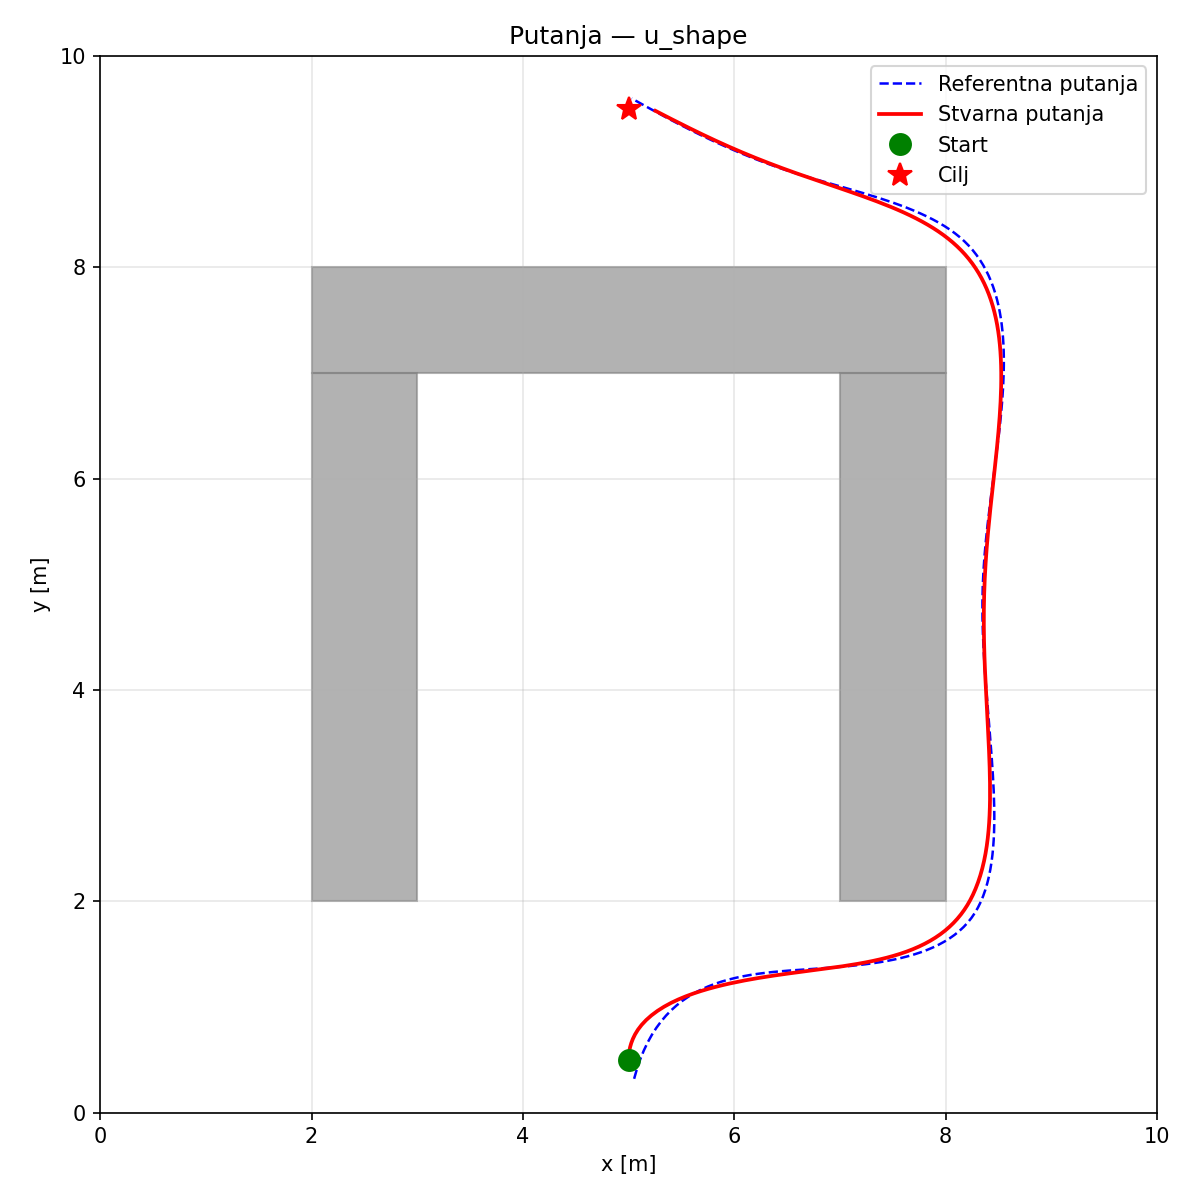
\includegraphics[width=0.82\linewidth]{figures/u_shape_traj.png}
  \caption{Referentna i stvarna putanja u scenariju U-oblika. A* planira put oko desne strane U-oblika, izbjegavajući slijepu ulicu.}
  \label{slk:ushape_traj}
\end{figure}

\begin{figure}[htbp]
  \centering
  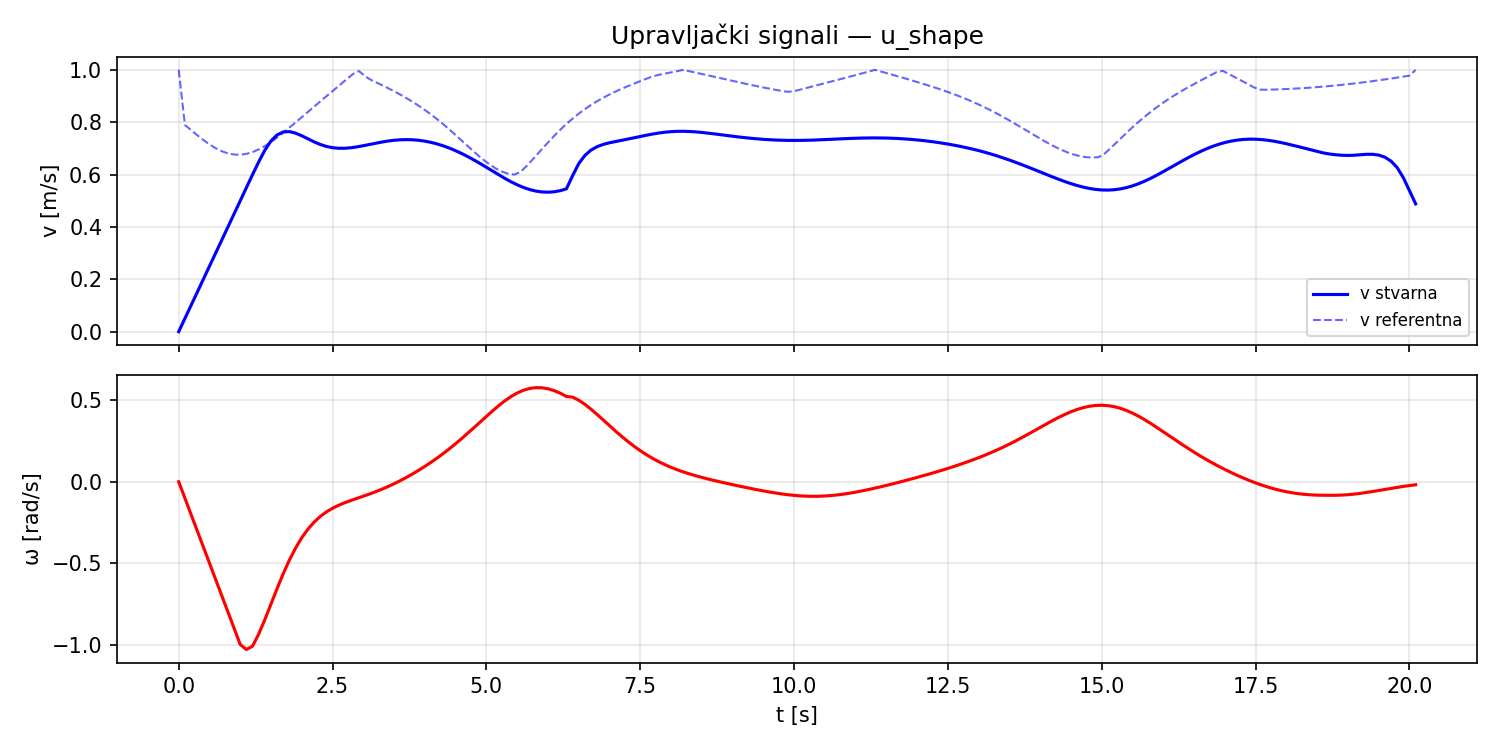
\includegraphics[width=0.82\linewidth]{figures/u_shape_controls.png}
  \caption{Upravljački profili u scenariju U-oblika. Tri vrha $\omega$ odgovaraju trima zavojima na putu oko U-oblika.}
  \label{slk:ushape_controls}
\end{figure}

\begin{figure}[htbp]
  \centering
  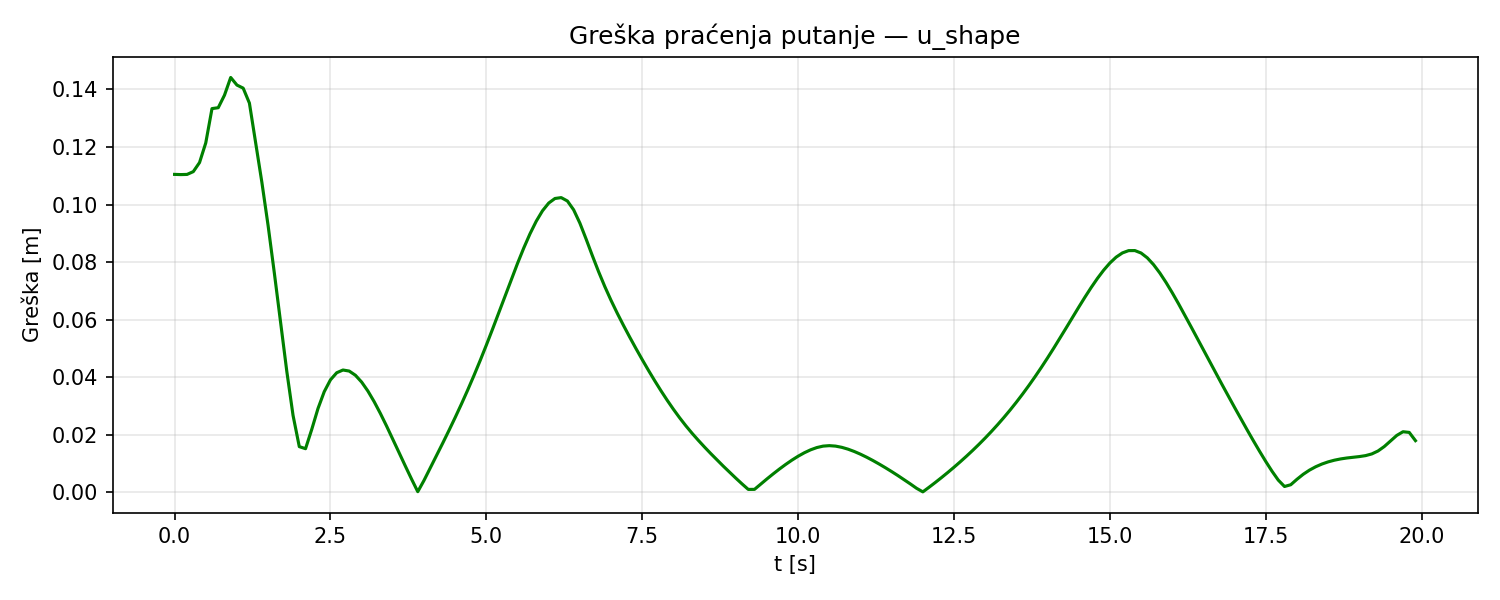
\includegraphics[width=0.82\linewidth]{figures/u_shape_error.png}
  \caption{Greška praćenja u scenariju U-oblika. Tri vrha greške odgovaraju trima zavojima putanje.}
  \label{slk:ushape_error}
\end{figure}

\begin{table}[H]
\centering
\caption{Metrike --- U-oblik}
\label{tab:ushape}
\begin{tabular}{lll}
\toprule
Metrika & Vrijednost & Usporedba s osnovnim \\
\midrule
RMSE & $0{,}0550$ m & $+59{,}8$\% \\
CTE srednji & $0{,}0400$ m & $+274{,}5$\% \\
CTE max & $0{,}1413$ m & $-4{,}4$\% \\
Greška smjera (srednja) & $3{,}19°$ & $+16{,}9$\% \\
Vrijeme do cilja & $20{,}10$ s & $+0{,}5$\% \\
CPU (prosjek / max) & $0{,}114$ ms / $0{,}270$ ms & $+25{,}3$\% \\
Dostigao cilj & Da & --- \\
\bottomrule
\end{tabular}
\end{table}

Uspješno dovršavanje ovog scenarija potvrđuje ispravnost dvoslojne arhitekture. RMSE od $55{,}0$ mm drugi je po redu (iza L-hodnika) jer svaki od tri zavoja nakratko podigne grešku, no između zavoja praćenje je na razini osnovnog scenarija.

\FloatBarrier
% ─────────────────────────────────────────────────────────────────────────────
\section{Poremećaj i oporavak}
\label{sec:r_perturbation}

Scenarij ispituje sposobnost oporavka sustava od nagle vanjske sile. Konfiguracija je identična osnovnom scenariju (ravna putanja od $(0{,}5;\; 5{,}0)$ do $(9{,}5;\; 5{,}0)$), s tom razlikom da se u koraku $k = 30$ ($t = 3{,}0$ s) stanje robota pomakne za $\Delta y = +1{,}0$ m. Poremećaj modelira nagli udarac --- događaj koji sustav ne može predvidjeti jer nije dio modela.

\begin{figure}[htbp]
  \centering
  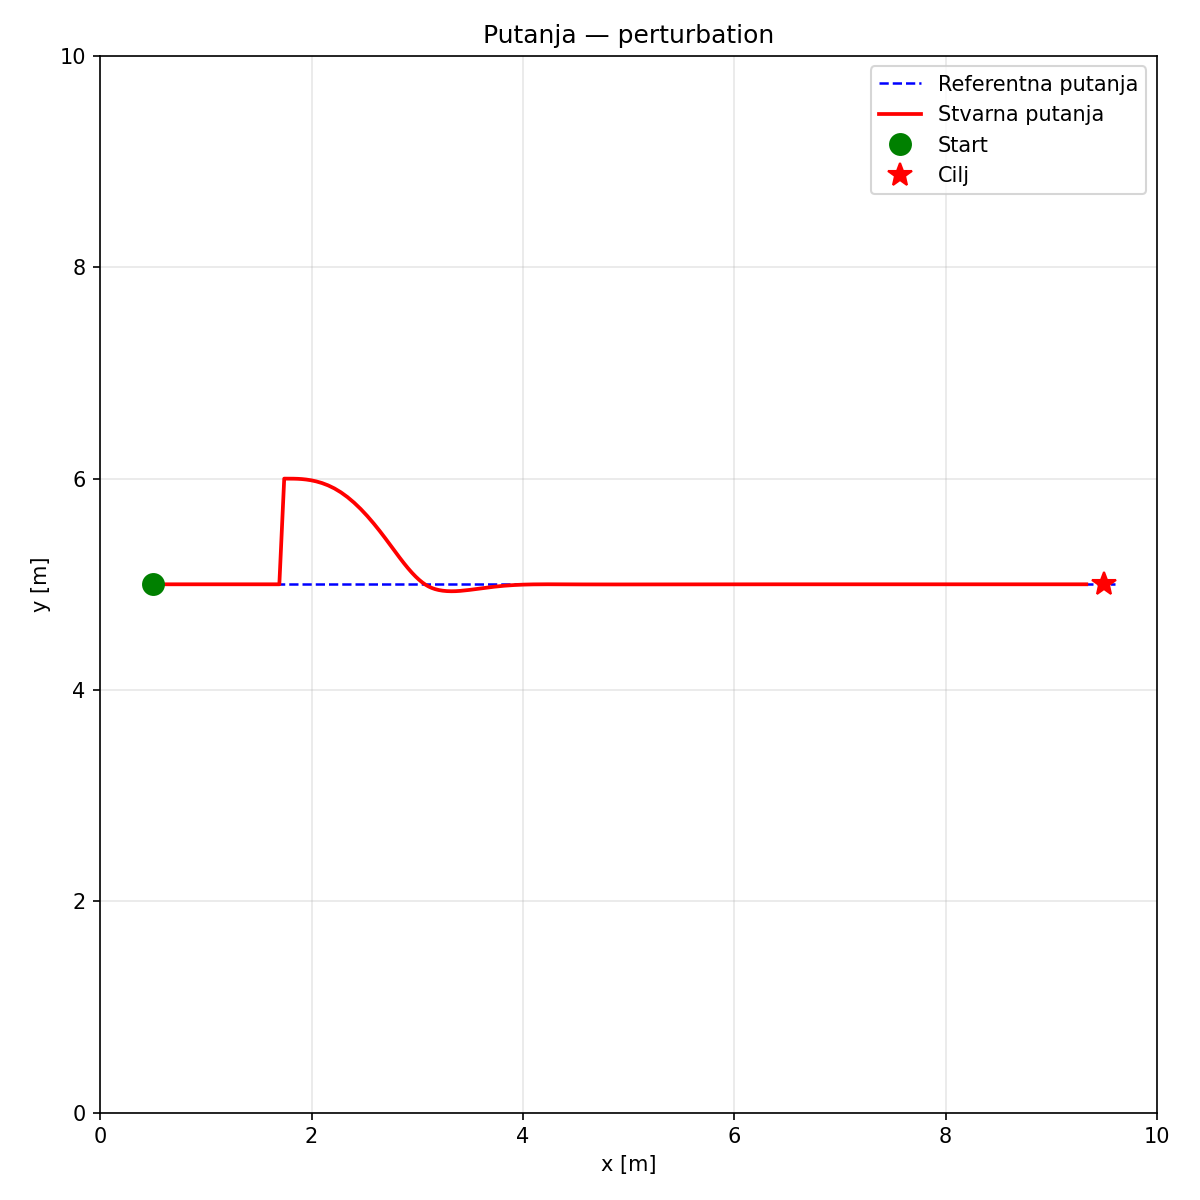
\includegraphics[width=0.82\linewidth]{figures/perturbation_traj.png}
  \caption{Referentna i stvarna putanja u scenariju s poremećajem. Nagli pomak za $1{,}0$ m vidljiv je kao karakteristični skok u trajektoriji, nakon kojega robot brzo vraća na referentnu putanju.}
  \label{slk:perturbation_traj}
\end{figure}

Do $t = 3{,}0$ s robot savršeno prati horizontalnu referencu. U trenutku poremećaja robot je transliran na $y \approx 6{,}0$ m. NMPC u sljedećem koraku prima stvarno stanje, vidi grešku od $1{,}0$ m i počinje ispravljati poziciju robota. Robot opisuje luk koji ga vraća prema referentnoj putanji i već pri $t \approx 5{,}2$ s ponovo se poravnava s referencom.

\begin{figure}[htbp]
  \centering
  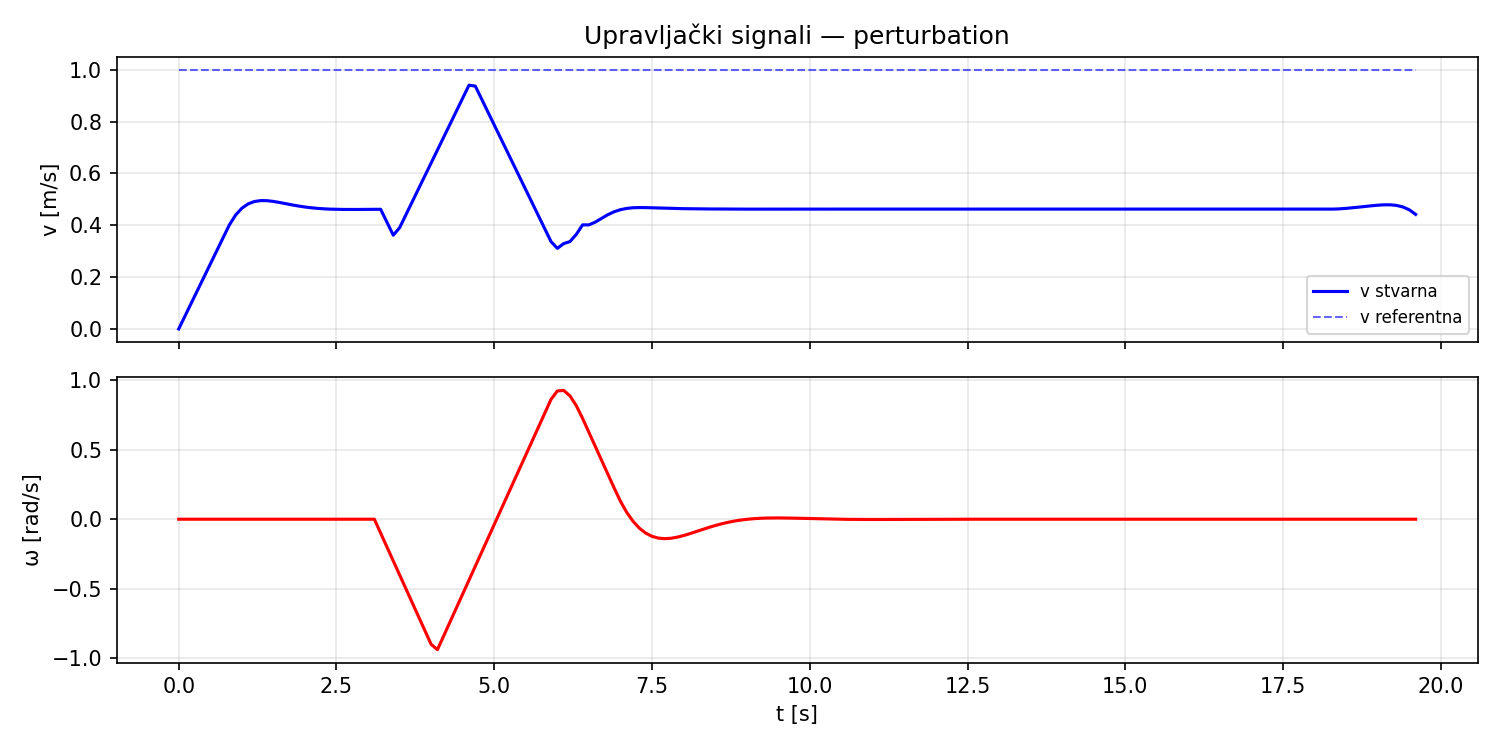
\includegraphics[width=0.82\linewidth]{figures/perturbation_controls.png}
  \caption{Upravljački signali u scenariju s poremećajem. Korektivni impulsi vidljivi su neposredno nakon $t = 3{,}0$ s.}
  \label{slk:perturbation_controls}
\end{figure}

\begin{figure}[htbp]
  \centering
  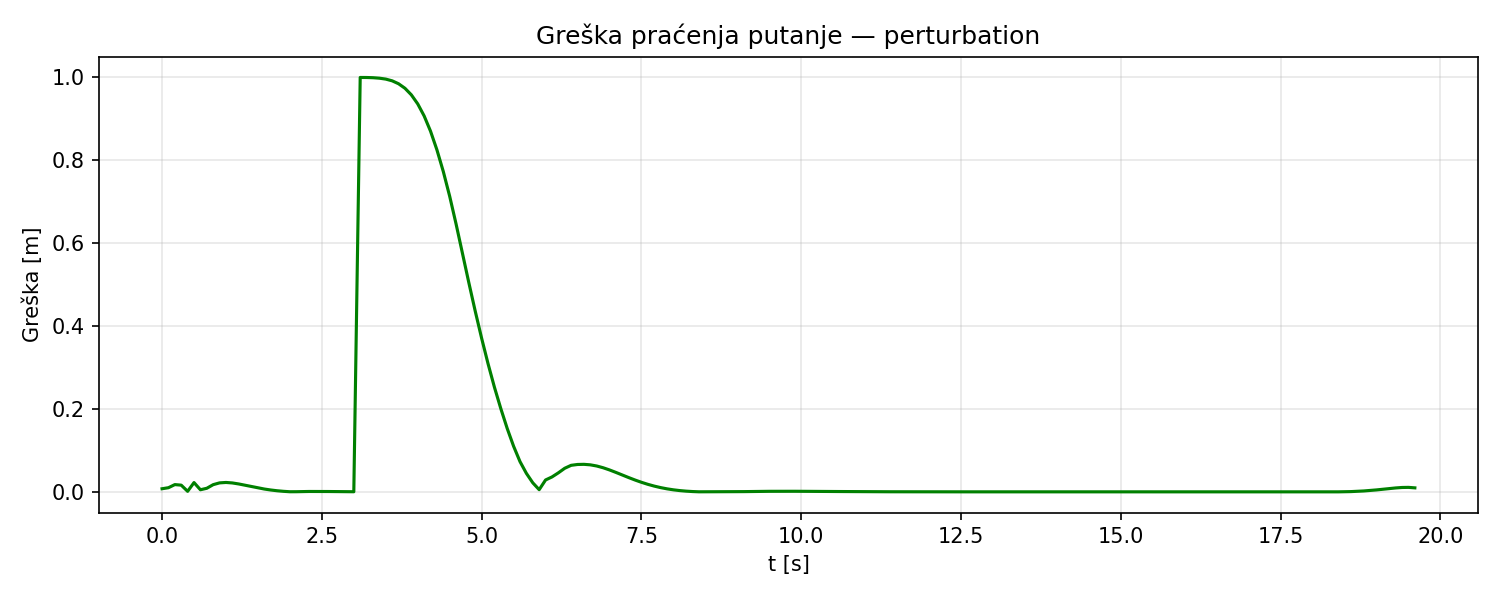
\includegraphics[width=0.82\linewidth]{figures/perturbation_error.png}
  \caption{Greška praćenja u scenariju s poremećajem. CTE skoči na $1{,}0$ m pri $t = 3{,}0$ s i vraća se ispod $0{,}3$ m unutar $22$ koraka ($2{,}2$ s).}
  \label{slk:perturbation_error}
\end{figure}

\begin{table}[H]
\centering
\caption{Metrike --- poremećaj}
\label{tab:perturbation}
\begin{tabular}{ll}
\toprule
Metrika & Vrijednost \\
\midrule
RMSE & $0{,}2736$ m \\
CTE srednji & $0{,}0942$ m \\
CTE max & $1{,}0000$ m \\
Greška smjera (srednja) & $5{,}68°$ \\
Trajanje oporavka (do greške $< 0{,}3$ m) & $22$ koraka ($2{,}2$ s) \\
Vrijeme do cilja & $19{,}60$ s \\
CPU (prosjek / max) & $0{,}118$ ms / $0{,}321$ ms \\
Dostigao cilj & Da \\
\bottomrule
\end{tabular}
\end{table}

Visoki RMSE ($273{,}6$ mm) posljedica je isključivo jednog trenutačnog poremećaja. Ključni zaključak jest da NMPC u zatvorenoj petlji automatski ispravlja poremećaje --- nije implementirana nikakva posebna logika za detekciju ili oporavak. Sustav na svakom koraku prima stvarno stanje i rješava OCP prema naprijed, što samo po sebi generira korektivne akcije.

\FloatBarrier
% ─────────────────────────────────────────────────────────────────────────────
\section{Gusti raspored prepreka}
\label{sec:r_cluttered}

Scenarij smješta sedam kružnih prepreka polumjera $0{,}6$--$0{,}8$ m na različite položaje u prostoru. Robot mora prijeći dijagonalnu putanju od $(0{,}5;\; 0{,}5)$ do $(9{,}5;\; 9{,}5)$. Scenarij testira skalabilnost sustava s povećanim brojem mekih ograničenja prepreka u OCP-u.

\begin{figure}[htbp]
  \centering
  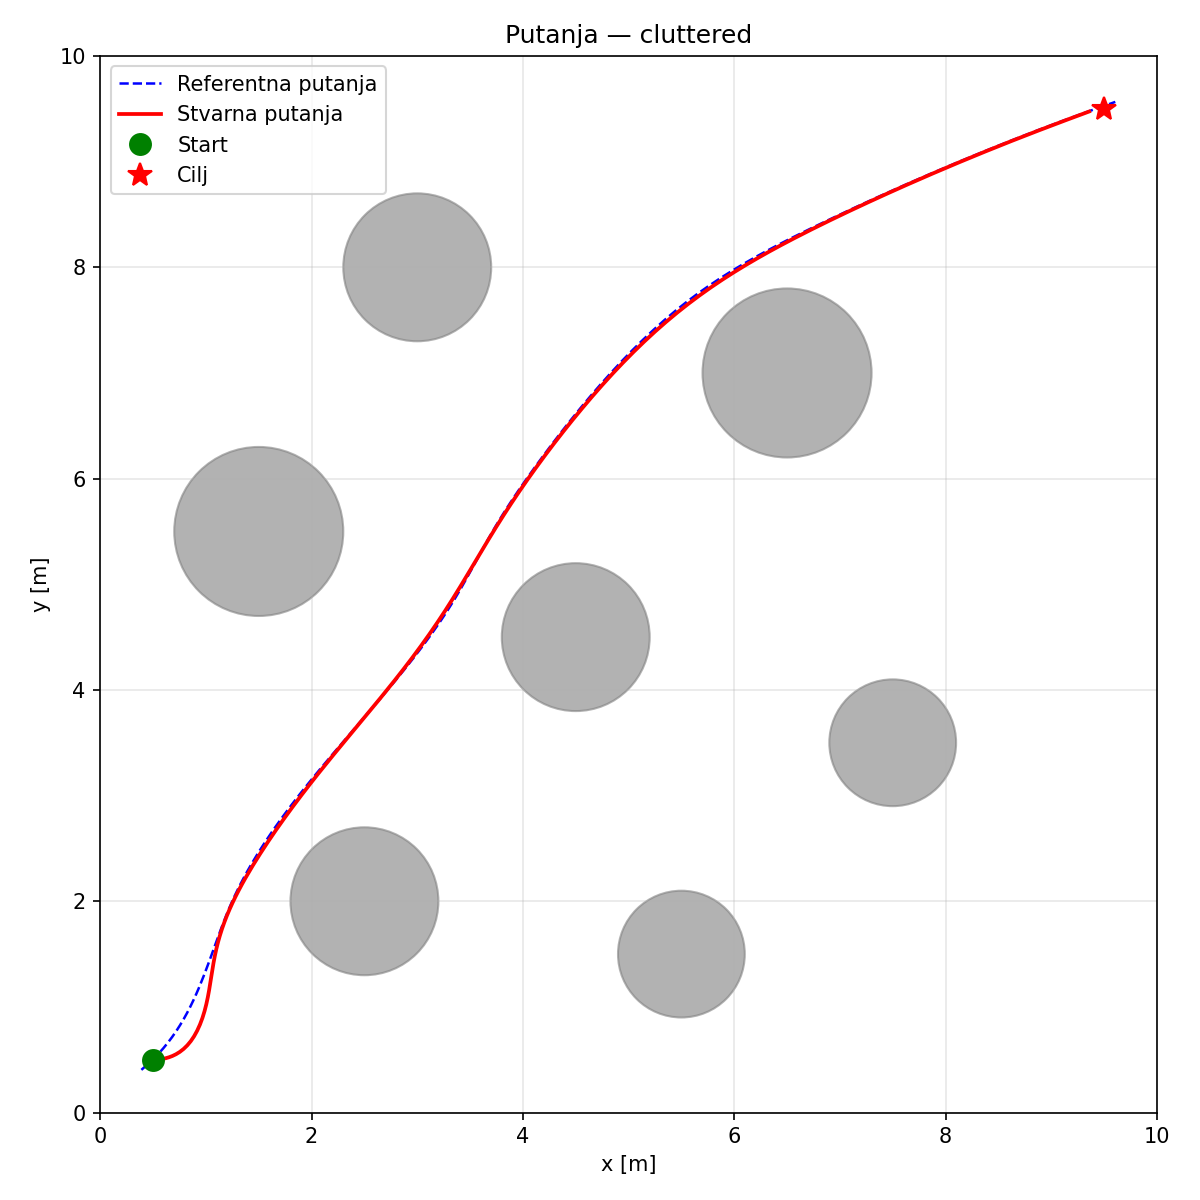
\includegraphics[width=0.82\linewidth]{figures/cluttered_traj.png}
  \caption{Referentna i stvarna putanja u scenariju gustog rasporeda prepreka. A* pronalazi glatku trajektoriju između svih sedam prepreka.}
  \label{slk:cluttered_traj}
\end{figure}

\begin{figure}[htbp]
  \centering
  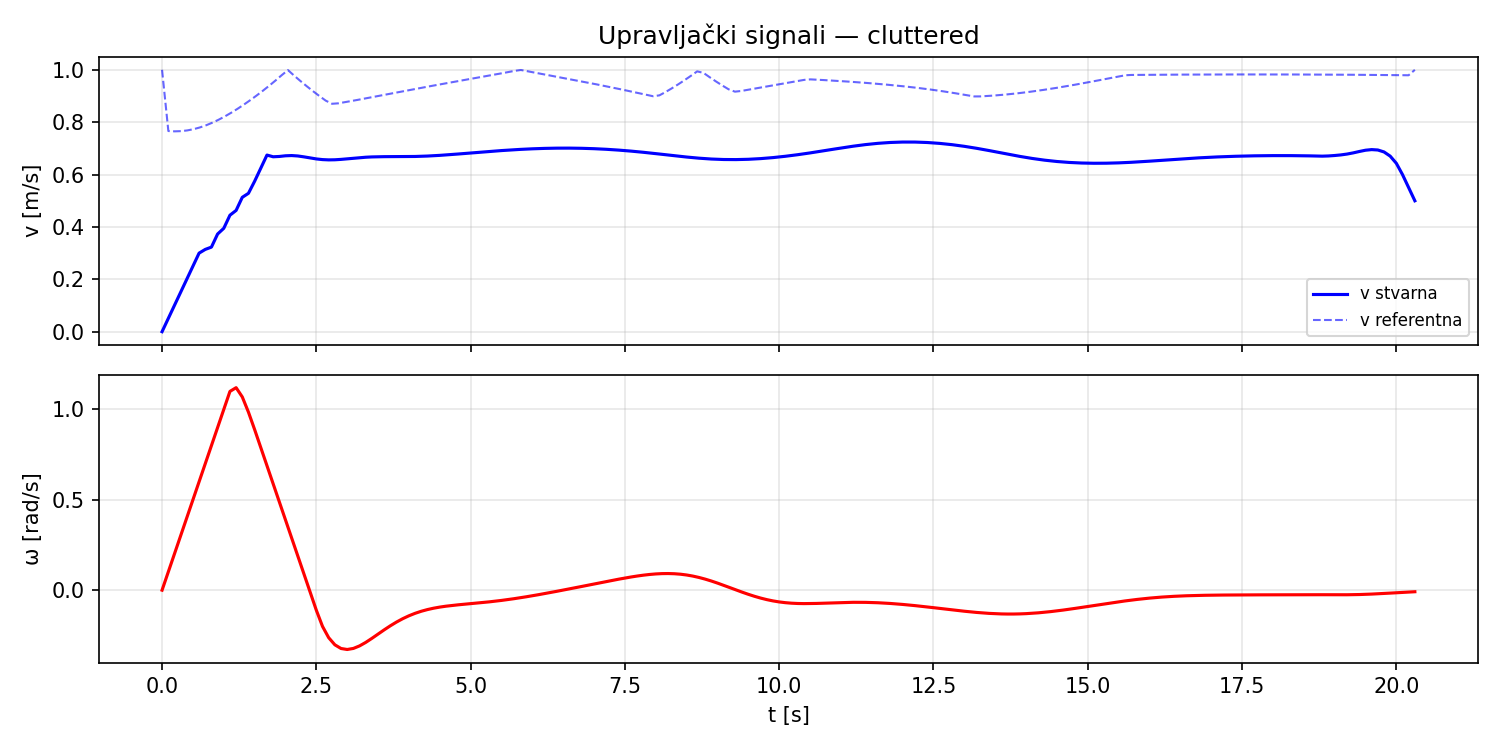
\includegraphics[width=0.82\linewidth]{figures/cluttered_controls.png}
  \caption{Upravljački profili u scenariju gustog rasporeda. Robot dosljedno održava brzinu oko $0{,}65$--$0{,}70$ m/s --- NMPC autonomno bira nižu brzinu pri navigaciji kroz zakrivljenu putanju.}
  \label{slk:cluttered_controls}
\end{figure}

Stvarna brzina dosljedno se zadržava ispod $v_{max} = 1{,}0$ m/s jer NMPC autonomno bira nižu brzinu pri navigaciji kroz zakrivljenu putanju između sedam prepreka.

\begin{figure}[htbp]
  \centering
  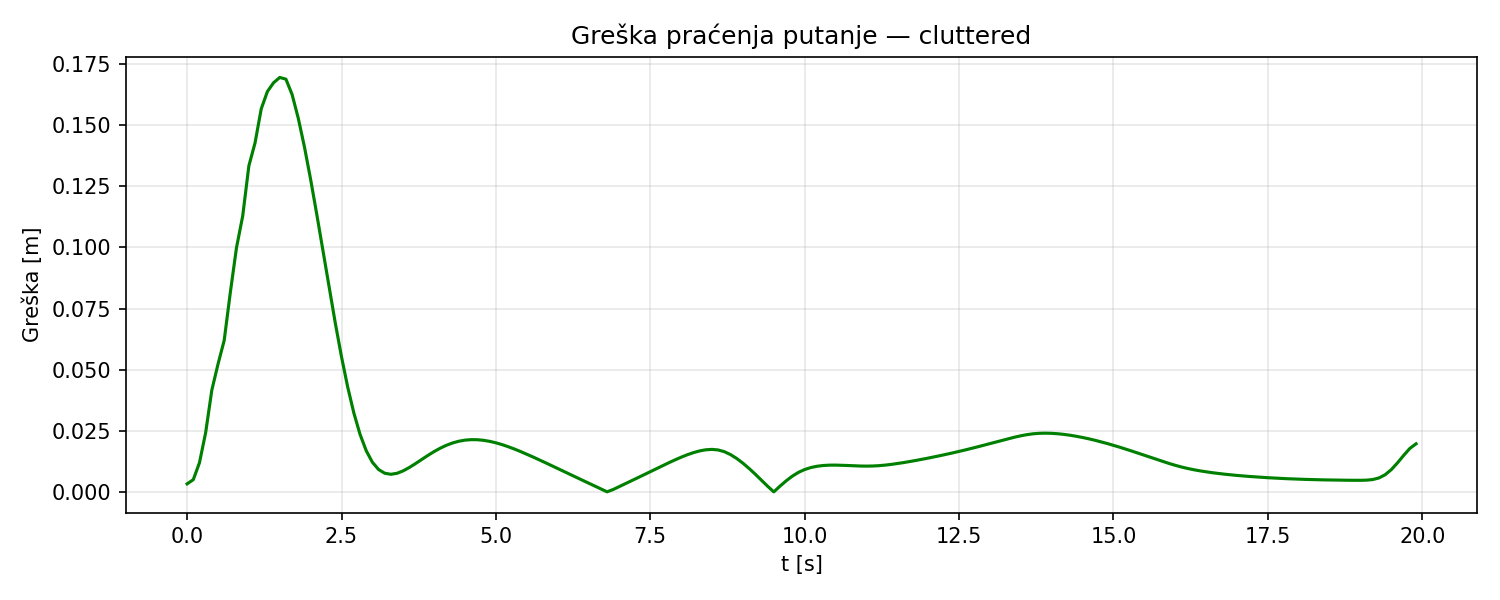
\includegraphics[width=0.82\linewidth]{figures/cluttered_error.png}
  \caption{Greška praćenja u scenariju gustog rasporeda. Nakon inicijalnog vrha, greška ostaje u rasponu $0{,}01$--$0{,}033$ m.}
  \label{slk:cluttered_error}
\end{figure}

\begin{table}[H]
\centering
\caption{Metrike --- gusti raspored prepreka}
\label{tab:cluttered}
\begin{tabular}{lll}
\toprule
Metrika & Vrijednost & Usporedba s osnovnim \\
\midrule
RMSE & $0{,}0429$ m & $+24{,}5$\% \\
CTE srednji & $0{,}0232$ m & $+116{,}9$\% \\
CTE max & $0{,}1678$ m & $+13{,}5$\% \\
Greška smjera (srednja) & $3{,}43°$ & $+25{,}8$\% \\
Broj prepreka & 7 & --- \\
Vrijeme do cilja & $20{,}30$ s & $+1{,}5$\% \\
CPU (prosjek / max) & $0{,}107$ ms / $0{,}277$ ms & $+17{,}6$\% \\
Dostigao cilj & Da & --- \\
\bottomrule
\end{tabular}
\end{table}

RMSE od $42{,}9$ mm je iznimno dobar rezultat za scenarij s najvećim brojem prepreka --- bolji od L-hodnika ($72{,}4$ mm) i U-oblika ($55{,}0$ mm). Razlog je glatka dijagonalna putanja bez naglih zavoja od $90°$. Dodatno CPU opterećenje od $17{,}6$\% u odnosu na osnovni scenarij potvrđuje da dodavanje sedam mekih ograničenja nema značajan utjecaj na računalni teret.

\FloatBarrier
% ─────────────────────────────────────────────────────────────────────────────
\section{Analiza osjetljivosti: predikcijski horizont $N$}
\label{sec:r_horizon}

Predikcijski horizont $N$ temeljni je projektni parametar koji definira broj koraka unaprijed u OCP-u. Duži horizont teorijski omogućuje bolju predikciju, ali povećava dimenzionalnost optimizacijskog problema i time računalni trošak. Analiza je provedena za $N \in \{5,\ 10,\ 15,\ 20,\ 30,\ 40\}$ na scenariju s jednom preprekom.

\begin{figure}[htbp]
  \centering
  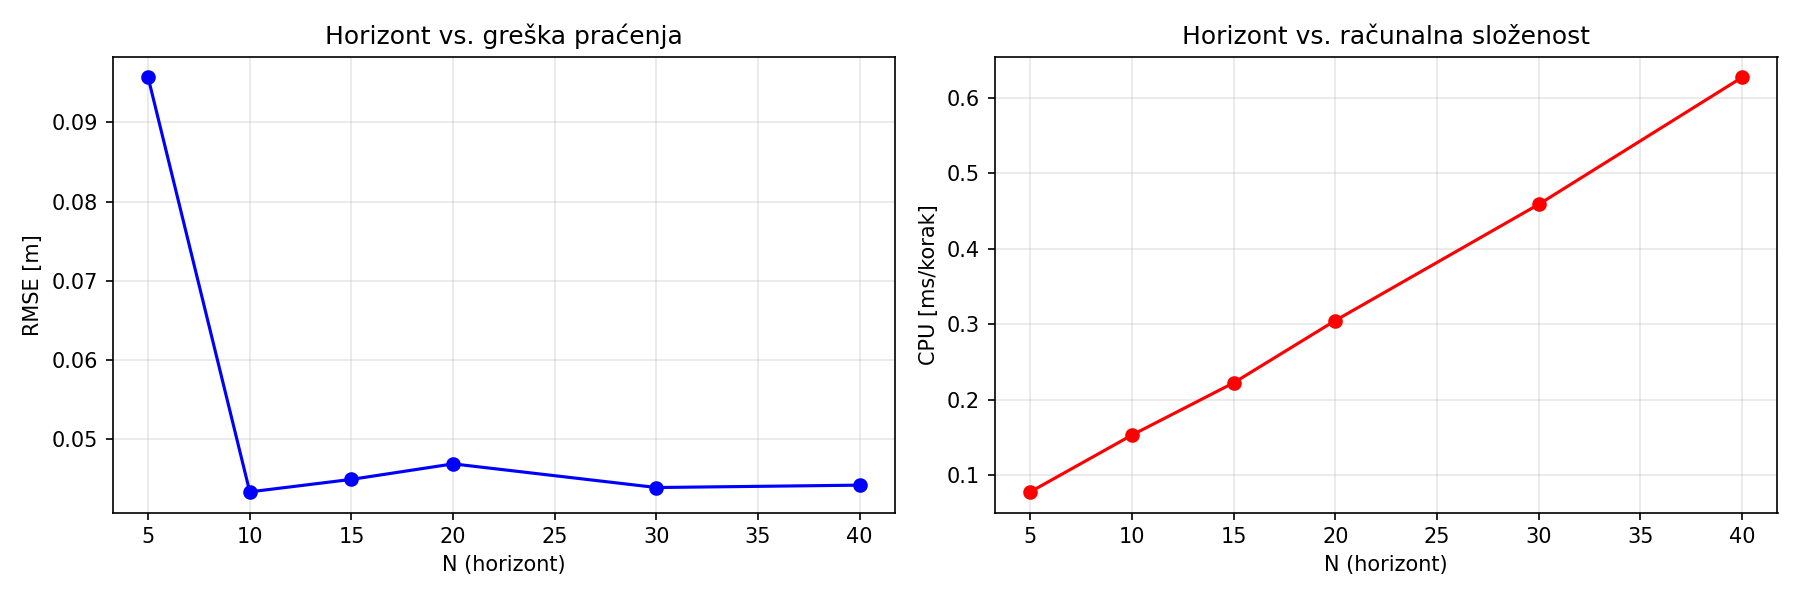
\includegraphics[width=0.95\linewidth]{figures/tuning_horizon.png}
  \caption{Greška praćenja (RMSE) i prosječno CPU vrijeme u ovisnosti o predikcijskom horizontu $N$. Zadana vrijednost $N = 20$ označena je kao referentna.}
  \label{slk:tuning_horizon}
\end{figure}

Rezultati na slici~\ref{slk:tuning_horizon} pokazuju tri zone:
\begin{itemize}
  \item \textbf{Kratki horizont ($N = 5$):} RMSE iznosi $95{,}7$ mm. Kratka predikcija ograničava predviđanje zakrivljene putanje izbjegavanja prepreke.
  \item \textbf{Prijelazna zona ($N = 10$--$20$):} RMSE naglo pada na $43{,}3$ mm pri $N = 10$, a zatim blago oscilira do $46{,}9$ mm pri $N = 20$.
  \item \textbf{Zasićena zona ($N = 30$--$40$):} RMSE se stabilizira na $\approx 44$ mm bez daljnjeg poboljšanja.
\end{itemize}

\begin{table}[H]
\centering
\caption{Kompromis preciznosti i CPU-a za različite horizonte}
\label{tab:horizon}
\begin{tabular}{llll}
\toprule
$N$ & RMSE [mm] & CPU prosjek [ms] & Normalizirani CPU \\
\midrule
5 & $95{,}7$ & $0{,}078$ & $1{,}0\times$ \\
10 & $43{,}3$ & $0{,}153$ & $2{,}0\times$ \\
15 & $44{,}9$ & $0{,}222$ & $2{,}9\times$ \\
\textbf{20} & $\mathbf{46{,}9}$ & $\mathbf{0{,}305}$ & $\mathbf{3{,}9\times}$ \\
30 & $43{,}9$ & $0{,}459$ & $5{,}9\times$ \\
40 & $44{,}2$ & $0{,}627$ & $8{,}1\times$ \\
\bottomrule
\end{tabular}
\end{table}

CPU raste gotovo linearno s $N$, što je konzistentno s teorijskim ponašanjem SQP\_RTI solvera čija složenost po iteraciji raste linearno s dimenzijom predikcijskog vektora. Odabir $N = 20$ temelji se na uravnoteženom kompromisu: u usporedbi s $N = 10$ postiže stabilniji RMSE, a u usporedbi s $N = 30$ razlika u RMSE manja je od $3$ mm uz $33$\% manji CPU.

\textbf{Napomena o metodološkoj razlici CPU vrijednosti.} Vrijednosti CPU-a u tablici~\ref{tab:horizon} ($0{,}078$--$0{,}627$ ms) veće su od vrijednosti u scenariju jedne prepreke (tablica~\ref{tab:one_obstacle}, $0{,}099$ ms za $N=20$) iako je RMSE identičan ($46{,}9$ mm). Razlog je metodološka razlika: analiza horizonta pokrenuta je kao zaseban skript koji za svaki $N$ iznova inicijalizira \texttt{AcadosOcpSolver} i generira novi C kod solvera. Svaka inicijalizacija uključuje hladan start (\textit{cold start}) predikcijskog modela bez prethodno zagrijane JIT/kompajlerske predmemorije. Scenarijska usporedba koristi već kompajlirani solver, čiji su SQP\_RTI pozivi brži zahvaljujući zagrijanju predmemorije instrukacija i podataka. Apsolutne vrijednosti u tablici~\ref{tab:horizon} treba tumačiti kao gornju granicu CPU-a za hladni start pri promjeni konfiguracije, a ne kao radne vrijednosti u normalnom radu.

\FloatBarrier
% ─────────────────────────────────────────────────────────────────────────────
\section{Analiza osjetljivosti: težine troška}
\label{sec:r_weights}

Omjer $Q/R$ temeljni je stupanj slobode koji određuje karakter NMPC-a: visoki $Q$ kažnjava grešku praćenja, visoki $R$ kažnjava agresivne promjene upravljanja. Testirana su četiri konfiguracijska profila uz konstantan $N = 20$:

\begin{figure}[htbp]
  \centering
  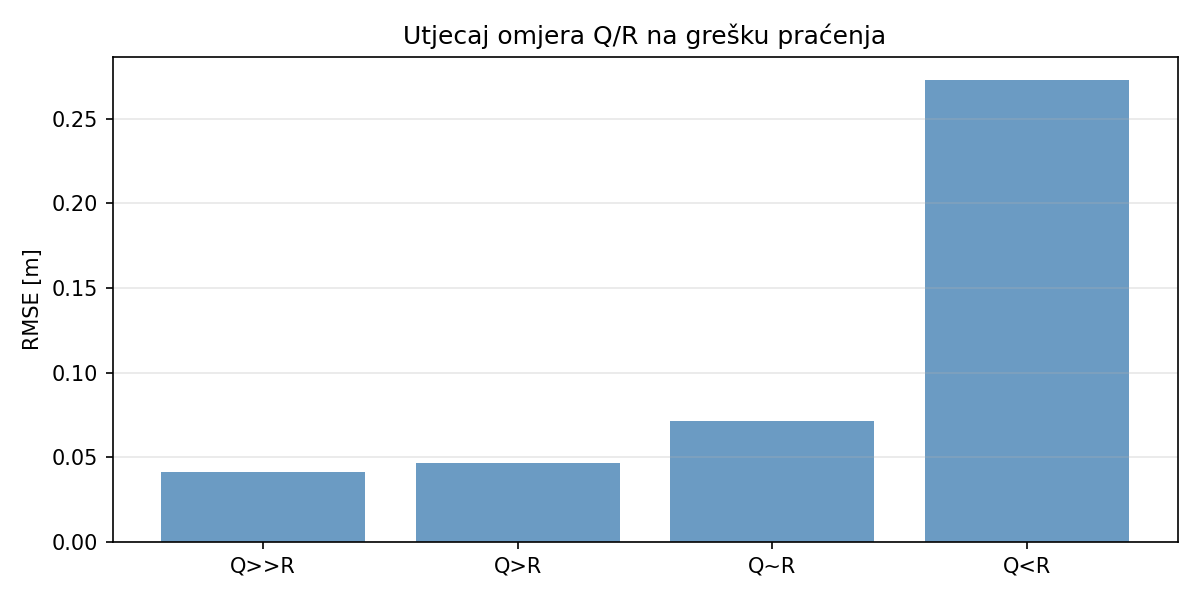
\includegraphics[width=0.82\linewidth]{figures/tuning_weights.png}
  \caption{RMSE praćenja za četiri konfiguracijska profila omjera $Q/R$ u scenariju jedne prepreke.}
  \label{slk:tuning_weights}
\end{figure}

\begin{table}[H]
\centering
\caption{Utjecaj konfiguracije težina na preciznost praćenja}
\label{tab:weights}
\begin{tabular}{lllll}
\toprule
Konfiguracija & $Q$ (pos.) & $R$ & RMSE [mm] & Karakter upravljanja \\
\midrule
Q$\gg$R & $50{,}0$ & $0{,}01$ & $41{,}5$ & Intenzivno, responzivno \\
\textbf{Q$>$R} & $\mathbf{10{,}0}$ & $\mathbf{0{,}1}$ & $\mathbf{46{,}9}$ & \textbf{Glatko, responzivno} \\
Q$\sim$R & $5{,}0$ & $1{,}0$ & $71{,}2$ & Slabije praćenje \\
Q$<$R & $1{,}0$ & $5{,}0$ & $272{,}9$ & Pasivno, neučinkovito \\
\bottomrule
\end{tabular}
\end{table}

Rezultati pokazuju monoton redoslijed: preciznost praćenja raste s porastom omjera $Q/R$. Konfiguracija Q$\gg$R postiže najmanji RMSE ($41{,}5$ mm), no po cijenu agresivnijih upravljačkih akcija. Konfiguracija Q$<$R ($Q = 1{,}0$, $R = 5{,}0$) postiže daleko najlošiji RMSE ($272{,}9$ mm) jer optimizator ``bira'' manje upravljačkih akcija kako bi smanjio trošak $R$, što rezultira trajnom velikom greškom pozicije.

Zadana konfiguracija $Q = 10{,}0$, $R = 0{,}1$ (omjer $100{:}1$) odabrana je kao optimalno kompromisno rješenje koje postiže RMSE od $46{,}9$ mm uz upravljačke signale dovoljno glatke za mehanički sustav.

\FloatBarrier
% ─────────────────────────────────────────────────────────────────────────────
\section{Zbirna usporedba scenarija}
\label{sec:r_summary}

Tablica~\ref{tab:summary} donosi objedinjeni pregled svih sedam testnih scenarija.

\begin{table}[H]
\centering
\caption{Zbirna tablica rezultata --- svi scenariji}
\label{tab:summary}
\small
\begin{tabular}{lllllll}
\toprule
Scenarij & RMSE [m] & CTE sred.\ [m] & Kut.\ greška [°] & Vrij.\ [s] & CPU prs.\ [ms] & Cilj \\
\midrule
Osnovna putanja   & $0{,}0344$ & $0{,}0107$ & $2{,}73$ & $20{,}0$ & $0{,}091$ & Da \\
Jedna prepreka    & $0{,}0469$ & $0{,}0278$ & $3{,}87$ & $20{,}0$ & $0{,}099$ & Da \\
Uski prolaz       & $0{,}0344$ & $0{,}0270$ & $1{,}59$ & $19{,}7$ & $0{,}089$ & Da \\
L-hodnik          & $0{,}0724$ & $0{,}0457$ & $4{,}90$ & $20{,}4$ & $0{,}103$ & Da \\
U-oblik           & $0{,}0550$ & $0{,}0400$ & $3{,}19$ & $20{,}1$ & $0{,}114$ & Da \\
Poremećaj         & $0{,}2736$ & $0{,}0942$ & $5{,}68$ & $19{,}6$ & $0{,}118$ & Da \\
Gusti raspored    & $0{,}0429$ & $0{,}0232$ & $3{,}43$ & $20{,}3$ & $0{,}107$ & Da \\
\bottomrule
\end{tabular}
\end{table}

Svi scenariji završavaju uspješnim dosezanjem cilja. Isključivanjem scenarija poremećaja, RMSE ostalih scenarija kreće se u rasponu od $34{,}4$ mm do $72{,}4$ mm (faktor $2{,}1\times$), što je izvrsna preciznost za sustav koji se kreće brzinom do $1$ m/s.

Prosječno CPU vrijeme iznosi između $0{,}089$ ms i $0{,}118$ ms, a maksimalni izmjereni korak traje $0{,}359$ ms --- što je oko $280\times$ brže od raspoloživog uzornog intervala od $100$ ms. Ovo eksperimentalno potvrđuje da je sustav primjenjiv u stvarnom vremenu i na hardveru s ograničenim procesorskim resursima. Budući da acados generira optimizirani C kod namijenjen ugradbenim sustavima, opravdano je očekivati prihvatljivo vrijeme izvođenja i na slabijem hardveru poput Raspberry Pi 4 --- no to nije eksperimentalno verificirano u ovom radu i ostavlja se za budući rad (poglavlje~\ref{pog:zakljucak}).


\FloatBarrier
% ─────────────────────────────────────────────────────────────────────────────
\section{Nedostižni cilj --- granice sustava}
\label{sec:r_blocked}

Scenarij \texttt{blocked} ispituje ponašanje sustava kada A* algoritam za planiranje putanje ne može pronaći putanju bez sudara s preprekama. Pet kružnih prepreka polumjera $1{,}5$ m postavljeno je u vertikalni niz duž $x = 5{,}0$ m, formirajući potpunu prepreku od $y = 0$ do $y = 10$ m.

Efektivni polumjer svake prepreke pri A* pretraživanju iznosi $r + d_{inf} = 1{,}5 + 0{,}4 = 1{,}9$ m. Razmak između susjednih centara od $2{,}5$ m manji je od $2 \times 1{,}9 = 3{,}8$ m, pa se inflirana područja potpuno preklapaju i formiraju neprobojni zid.

\begin{figure}[H]
  \centering
  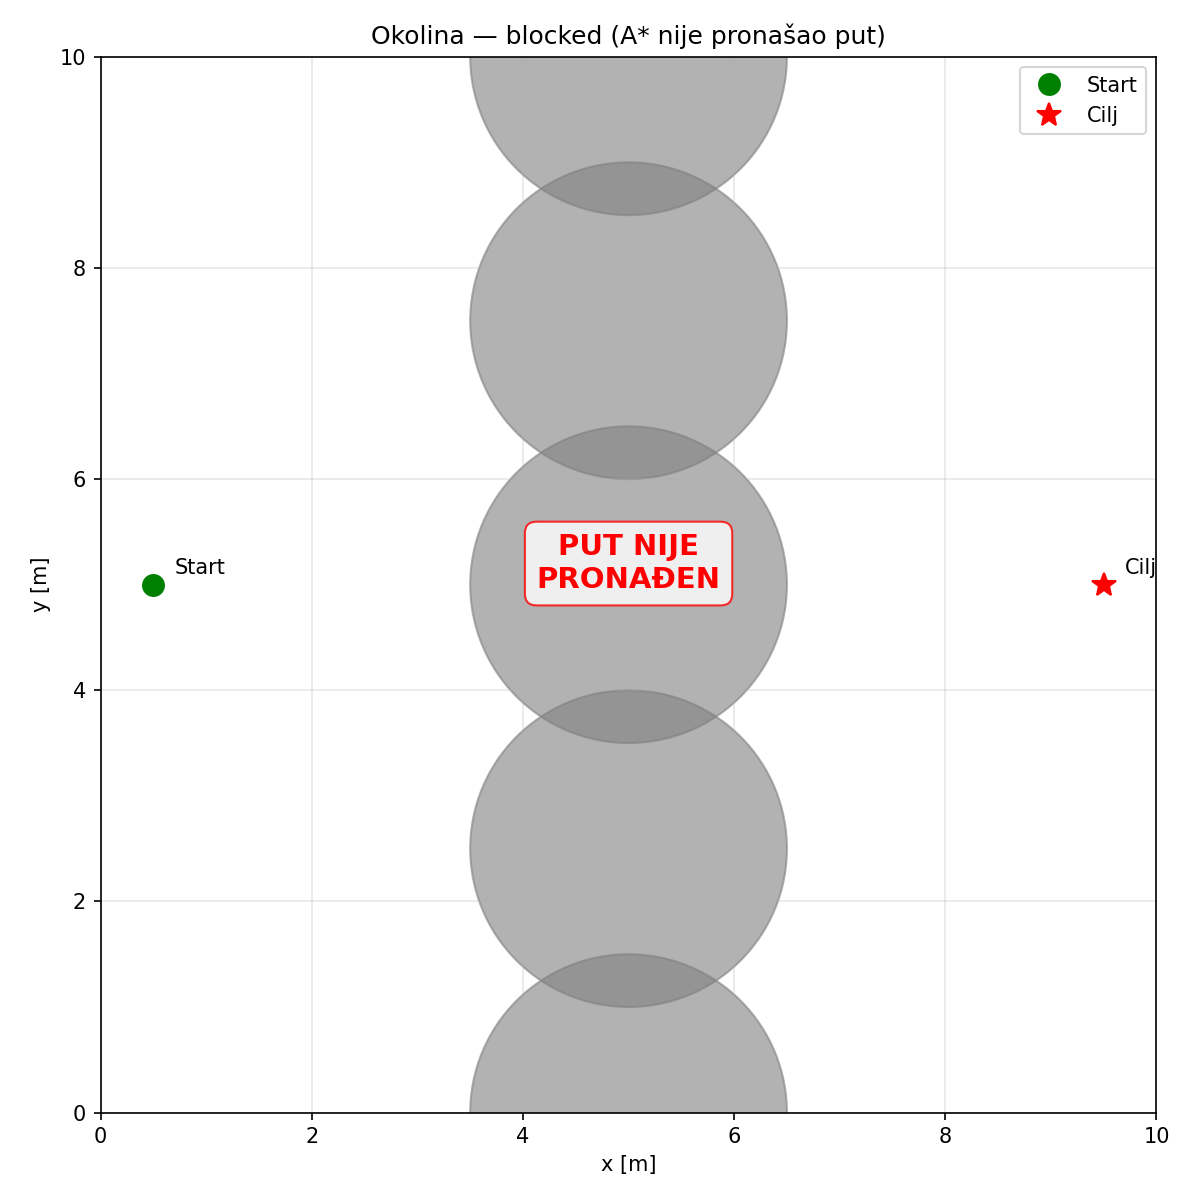
\includegraphics[width=0.82\linewidth]{figures/blocked_env.png}
  \caption{Vizualizacija blokirane okoline. Pet kružnih prepreka formira vertikalni zid koji potpuno blokira putanju od starta (lijevo) do cilja (desno).}
  \label{slk:blocked_env}
\end{figure}

A* ne pronalazi put i ispravno detektira neizvedivost --- heuristika ga vodi sve dok ne iscrpi sve dostupne čvorove na strani starta:

\begin{listing}[H]
\begin{minted}{bash}
RuntimeError: A*: nema puta od starta do cilja
\end{minted}
\caption{Poruka sustava pri nedostižnom cilju}
\end{listing}

Budući da referentna putanja nije generirana, NMPC solver se uopće ne pokreće. Ovo je ispravno ponašanje: A* algoritam djeluje kao \emph{filter izvedivosti} koji detektira neriješivost na razini planiranja, što je računalno učinkovito i arhitekturno ispravno.

